% Options for packages loaded elsewhere
\PassOptionsToPackage{unicode}{hyperref}
\PassOptionsToPackage{hyphens}{url}
\PassOptionsToPackage{dvipsnames,svgnames,x11names}{xcolor}
%
\documentclass[
  a4paperpaper,
]{article}

\usepackage{amsmath,amssymb}
\usepackage{iftex}
\ifPDFTeX
  \usepackage[T1]{fontenc}
  \usepackage[utf8]{inputenc}
  \usepackage{textcomp} % provide euro and other symbols
\else % if luatex or xetex
  \ifXeTeX
    \usepackage{mathspec} % this also loads fontspec
  \else
    \usepackage{unicode-math} % this also loads fontspec
  \fi
  \defaultfontfeatures{Scale=MatchLowercase}
  \defaultfontfeatures[\rmfamily]{Ligatures=TeX,Scale=1}
\fi
\usepackage{lmodern}
\ifPDFTeX\else  
    % xetex/luatex font selection
\fi
% Use upquote if available, for straight quotes in verbatim environments
\IfFileExists{upquote.sty}{\usepackage{upquote}}{}
\IfFileExists{microtype.sty}{% use microtype if available
  \usepackage[]{microtype}
  \UseMicrotypeSet[protrusion]{basicmath} % disable protrusion for tt fonts
}{}
\makeatletter
\@ifundefined{KOMAClassName}{% if non-KOMA class
  \IfFileExists{parskip.sty}{%
    \usepackage{parskip}
  }{% else
    \setlength{\parindent}{0pt}
    \setlength{\parskip}{6pt plus 2pt minus 1pt}}
}{% if KOMA class
  \KOMAoptions{parskip=half}}
\makeatother
\usepackage{xcolor}
\setlength{\emergencystretch}{3em} % prevent overfull lines
\setcounter{secnumdepth}{-\maxdimen} % remove section numbering
% Make \paragraph and \subparagraph free-standing
\ifx\paragraph\undefined\else
  \let\oldparagraph\paragraph
  \renewcommand{\paragraph}[1]{\oldparagraph{#1}\mbox{}}
\fi
\ifx\subparagraph\undefined\else
  \let\oldsubparagraph\subparagraph
  \renewcommand{\subparagraph}[1]{\oldsubparagraph{#1}\mbox{}}
\fi

\usepackage{color}
\usepackage{fancyvrb}
\newcommand{\VerbBar}{|}
\newcommand{\VERB}{\Verb[commandchars=\\\{\}]}
\DefineVerbatimEnvironment{Highlighting}{Verbatim}{commandchars=\\\{\}}
% Add ',fontsize=\small' for more characters per line
\usepackage{framed}
\definecolor{shadecolor}{RGB}{241,243,245}
\newenvironment{Shaded}{\begin{snugshade}}{\end{snugshade}}
\newcommand{\AlertTok}[1]{\textcolor[rgb]{0.68,0.00,0.00}{#1}}
\newcommand{\AnnotationTok}[1]{\textcolor[rgb]{0.37,0.37,0.37}{#1}}
\newcommand{\AttributeTok}[1]{\textcolor[rgb]{0.40,0.45,0.13}{#1}}
\newcommand{\BaseNTok}[1]{\textcolor[rgb]{0.68,0.00,0.00}{#1}}
\newcommand{\BuiltInTok}[1]{\textcolor[rgb]{0.00,0.23,0.31}{#1}}
\newcommand{\CharTok}[1]{\textcolor[rgb]{0.13,0.47,0.30}{#1}}
\newcommand{\CommentTok}[1]{\textcolor[rgb]{0.37,0.37,0.37}{#1}}
\newcommand{\CommentVarTok}[1]{\textcolor[rgb]{0.37,0.37,0.37}{\textit{#1}}}
\newcommand{\ConstantTok}[1]{\textcolor[rgb]{0.56,0.35,0.01}{#1}}
\newcommand{\ControlFlowTok}[1]{\textcolor[rgb]{0.00,0.23,0.31}{#1}}
\newcommand{\DataTypeTok}[1]{\textcolor[rgb]{0.68,0.00,0.00}{#1}}
\newcommand{\DecValTok}[1]{\textcolor[rgb]{0.68,0.00,0.00}{#1}}
\newcommand{\DocumentationTok}[1]{\textcolor[rgb]{0.37,0.37,0.37}{\textit{#1}}}
\newcommand{\ErrorTok}[1]{\textcolor[rgb]{0.68,0.00,0.00}{#1}}
\newcommand{\ExtensionTok}[1]{\textcolor[rgb]{0.00,0.23,0.31}{#1}}
\newcommand{\FloatTok}[1]{\textcolor[rgb]{0.68,0.00,0.00}{#1}}
\newcommand{\FunctionTok}[1]{\textcolor[rgb]{0.28,0.35,0.67}{#1}}
\newcommand{\ImportTok}[1]{\textcolor[rgb]{0.00,0.46,0.62}{#1}}
\newcommand{\InformationTok}[1]{\textcolor[rgb]{0.37,0.37,0.37}{#1}}
\newcommand{\KeywordTok}[1]{\textcolor[rgb]{0.00,0.23,0.31}{#1}}
\newcommand{\NormalTok}[1]{\textcolor[rgb]{0.00,0.23,0.31}{#1}}
\newcommand{\OperatorTok}[1]{\textcolor[rgb]{0.37,0.37,0.37}{#1}}
\newcommand{\OtherTok}[1]{\textcolor[rgb]{0.00,0.23,0.31}{#1}}
\newcommand{\PreprocessorTok}[1]{\textcolor[rgb]{0.68,0.00,0.00}{#1}}
\newcommand{\RegionMarkerTok}[1]{\textcolor[rgb]{0.00,0.23,0.31}{#1}}
\newcommand{\SpecialCharTok}[1]{\textcolor[rgb]{0.37,0.37,0.37}{#1}}
\newcommand{\SpecialStringTok}[1]{\textcolor[rgb]{0.13,0.47,0.30}{#1}}
\newcommand{\StringTok}[1]{\textcolor[rgb]{0.13,0.47,0.30}{#1}}
\newcommand{\VariableTok}[1]{\textcolor[rgb]{0.07,0.07,0.07}{#1}}
\newcommand{\VerbatimStringTok}[1]{\textcolor[rgb]{0.13,0.47,0.30}{#1}}
\newcommand{\WarningTok}[1]{\textcolor[rgb]{0.37,0.37,0.37}{\textit{#1}}}

\providecommand{\tightlist}{%
  \setlength{\itemsep}{0pt}\setlength{\parskip}{0pt}}\usepackage{longtable,booktabs,array}
\usepackage{calc} % for calculating minipage widths
% Correct order of tables after \paragraph or \subparagraph
\usepackage{etoolbox}
\makeatletter
\patchcmd\longtable{\par}{\if@noskipsec\mbox{}\fi\par}{}{}
\makeatother
% Allow footnotes in longtable head/foot
\IfFileExists{footnotehyper.sty}{\usepackage{footnotehyper}}{\usepackage{footnote}}
\makesavenoteenv{longtable}
\usepackage{graphicx}
\makeatletter
\def\maxwidth{\ifdim\Gin@nat@width>\linewidth\linewidth\else\Gin@nat@width\fi}
\def\maxheight{\ifdim\Gin@nat@height>\textheight\textheight\else\Gin@nat@height\fi}
\makeatother
% Scale images if necessary, so that they will not overflow the page
% margins by default, and it is still possible to overwrite the defaults
% using explicit options in \includegraphics[width, height, ...]{}
\setkeys{Gin}{width=\maxwidth,height=\maxheight,keepaspectratio}
% Set default figure placement to htbp
\makeatletter
\def\fps@figure{htbp}
\makeatother

\usepackage{fvextra}
\DefineVerbatimEnvironment{Highlighting}{Verbatim}{breaklines,commandchars=\\\{\}}
\DefineVerbatimEnvironment{OutputCode}{Verbatim}{breaklines,commandchars=\\\{\}}
\makeatletter
\@ifpackageloaded{caption}{}{\usepackage{caption}}
\AtBeginDocument{%
\ifdefined\contentsname
  \renewcommand*\contentsname{Índice}
\else
  \newcommand\contentsname{Índice}
\fi
\ifdefined\listfigurename
  \renewcommand*\listfigurename{Lista de Figuras}
\else
  \newcommand\listfigurename{Lista de Figuras}
\fi
\ifdefined\listtablename
  \renewcommand*\listtablename{Lista de Tabelas}
\else
  \newcommand\listtablename{Lista de Tabelas}
\fi
\ifdefined\figurename
  \renewcommand*\figurename{Figura}
\else
  \newcommand\figurename{Figura}
\fi
\ifdefined\tablename
  \renewcommand*\tablename{Tabela}
\else
  \newcommand\tablename{Tabela}
\fi
}
\@ifpackageloaded{float}{}{\usepackage{float}}
\floatstyle{ruled}
\@ifundefined{c@chapter}{\newfloat{codelisting}{h}{lop}}{\newfloat{codelisting}{h}{lop}[chapter]}
\floatname{codelisting}{Listagem}
\newcommand*\listoflistings{\listof{codelisting}{Lista de Listagens}}
\makeatother
\makeatletter
\makeatother
\makeatletter
\@ifpackageloaded{caption}{}{\usepackage{caption}}
\@ifpackageloaded{subcaption}{}{\usepackage{subcaption}}
\makeatother
\ifLuaTeX
\usepackage[bidi=basic]{babel}
\else
\usepackage[bidi=default]{babel}
\fi
\babelprovide[main,import]{portuguese}
% get rid of language-specific shorthands (see #6817):
\let\LanguageShortHands\languageshorthands
\def\languageshorthands#1{}
\ifLuaTeX
  \usepackage{selnolig}  % disable illegal ligatures
\fi
\usepackage{bookmark}

\IfFileExists{xurl.sty}{\usepackage{xurl}}{} % add URL line breaks if available
\urlstyle{same} % disable monospaced font for URLs
\hypersetup{
  pdftitle={Lista 1: Ajustando uma RNA `no braço'},
  pdfauthor={César A. Galvão - 190011572},
  pdflang={pt},
  colorlinks=true,
  linkcolor={blue},
  filecolor={Maroon},
  citecolor={Blue},
  urlcolor={Blue},
  pdfcreator={LaTeX via pandoc}}

\title{Lista 1: Ajustando uma RNA `no braço'}
\author{César A. Galvão - 190011572}
\date{}

\begin{document}
\maketitle

Para essa lista, é considerada a seguinte arquitetura de uma rede neural
\emph{feed-forward}:\footnote{Documento disponível no repositório do
  autor: \url{https://github.com/cesar-galvao/Topicos-1---Redes-neurais}}

\begin{figure}[H]

{\centering 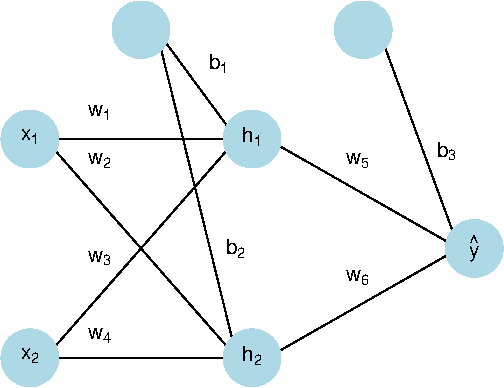
\includegraphics{lista1-resolucao_files/figure-pdf/figf-arquitetura-rede-1.pdf}

}

\caption{Arquitetura da rede neural artificial. Adotamos função de
ativação sigmoide e linear nas camadas escondidas e de saída,
respectivamente.}

\end{figure}%

\section{Questão 1}\label{questuxe3o-1}

\subsection{Item a}\label{item-a}

Crie uma função computacional para calcular o valor previso da variável
resposta \(\hat{y} = f(\boldsymbol{x}; \boldsymbol{\theta})\) em função
de \(\boldsymbol{x}\) e \(\boldsymbol{\theta}\). Use a função para
calcular \(\hat{y}\) para \(\boldsymbol{\theta} = (0.1, \dots , 0.1)\) e
\(\boldsymbol{x} = (1, 1)\).

\begin{center}\rule{0.5\linewidth}{0.5pt}\end{center}

Implementa-se de forma matricial. A função não é adaptativa ao tamanho
da rede e exige que o usuário forneça uma lista \(\boldsymbol{\theta}\)
com os seguintes elementos:

\begin{enumerate}
\def\labelenumi{\arabic{enumi}.}
\tightlist
\item
  \(W^{(1)}\) - matriz \(2 \times 2\) de pesos da camada de entrada
  \(\begin{pmatrix} w_1 & w_2 \\ w_3 & w_4 \end{pmatrix}\). Cada linha
  deve representar os pesos de cada neurônio para o neurônio
  subsequente, i.e.~\(w_{ij}\) representa o peso do neurônio de entrada
  \(i\) para o próximo neurônio \(j\).
\item
  \(\boldsymbol{b}^{(1)}\) - vetor de viés da camada de entrada
  \(\begin{pmatrix} b_1 \\ b_2 \end{pmatrix}\).
\item
  \(W^{(2)}\) - matriz \(2 \times 1\) de pesos da camada de saída
  \(\begin{pmatrix} w_5 \\ w_6 \end{pmatrix}\).
\item
  \(\boldsymbol{b}^{(2)}\) - vetor elemento de viés da camada de saída
  \(\begin{pmatrix} b_3 \end{pmatrix}\).
\end{enumerate}

Como função de ativação foi escolhida a função sigmóide denotada por
\(\phi = \frac{1}{1+e^{-x}}\). A função de previsão é dada por:

\[
\hat{y} = W^{(2)\top}\phi(W^{(1)\top}\boldsymbol{x} + \boldsymbol{b}^{(1)}) + \boldsymbol{b}^{(2)}
\]

ou

\begin{align*}
\boldsymbol{a} =& W^{(1)\top} \boldsymbol{x} + \boldsymbol{b^{(1)}} \\
\boldsymbol{h} =& \phi(\boldsymbol{a}) \\
\hat{y} =& W^{(2)\top}\boldsymbol{h} + b^{(2)}
\end{align*}

\begin{Shaded}
\begin{Highlighting}[]
\CommentTok{\# Função de ativação}
\NormalTok{phi }\OtherTok{\textless{}{-}} \ControlFlowTok{function}\NormalTok{(x) \{}\DecValTok{1}\SpecialCharTok{/}\NormalTok{(}\DecValTok{1} \SpecialCharTok{+} \FunctionTok{exp}\NormalTok{(}\SpecialCharTok{{-}}\NormalTok{x))\}}

\CommentTok{\# Função de previsão}
\NormalTok{ffwd }\OtherTok{\textless{}{-}} \ControlFlowTok{function}\NormalTok{(x, theta) \{}
  
  \ControlFlowTok{if}\NormalTok{(}\FunctionTok{any}\NormalTok{(}\FunctionTok{dim}\NormalTok{(theta[[}\DecValTok{1}\NormalTok{]]) }\SpecialCharTok{!=} \FunctionTok{c}\NormalTok{(}\DecValTok{2}\NormalTok{, }\DecValTok{2}\NormalTok{)))\{}
    \FunctionTok{stop}\NormalTok{(}\StringTok{"Feed Forward: O primeiro elemento de theta deve ser uma matriz de pesos 2x2 para a aplicação nos dados"}\NormalTok{)}
\NormalTok{  \} }\ControlFlowTok{else} \ControlFlowTok{if}\NormalTok{(}\FunctionTok{length}\NormalTok{(theta[[}\DecValTok{2}\NormalTok{]]) }\SpecialCharTok{!=} \DecValTok{2}\NormalTok{)\{}
    \FunctionTok{stop}\NormalTok{(}\StringTok{"Feed Forward: O segundo elemento de theta deve ser um vetor viés de tamanho 2 para somar aos dados"}\NormalTok{)}
\NormalTok{  \} }\ControlFlowTok{else} \ControlFlowTok{if}\NormalTok{(}\FunctionTok{any}\NormalTok{(}\FunctionTok{dim}\NormalTok{(theta[[}\DecValTok{3}\NormalTok{]]) }\SpecialCharTok{!=} \FunctionTok{c}\NormalTok{(}\DecValTok{2}\NormalTok{, }\DecValTok{1}\NormalTok{)))\{}
    \FunctionTok{stop}\NormalTok{(}\StringTok{"Feed Forward: O terceiro elemento de theta deve ser uma matriz de pesos 2x1 para aplicação na única camada h"}\NormalTok{)}
\NormalTok{  \} }\ControlFlowTok{else} \ControlFlowTok{if}\NormalTok{(}\FunctionTok{length}\NormalTok{(theta[[}\DecValTok{4}\NormalTok{]]) }\SpecialCharTok{!=} \DecValTok{1}\NormalTok{)\{}
    \FunctionTok{stop}\NormalTok{(}\StringTok{"Feed Forward: O quarto elemento de theta deve ser um vetor viés de tamanho 1 para soma na única camada h"}\NormalTok{)}
\NormalTok{  \} }\ControlFlowTok{else} \ControlFlowTok{if}\NormalTok{(}\SpecialCharTok{!}\FunctionTok{is.data.frame}\NormalTok{(x) }\SpecialCharTok{|} \SpecialCharTok{!}\NormalTok{tibble}\SpecialCharTok{::}\FunctionTok{is\_tibble}\NormalTok{(x) }\SpecialCharTok{\&} \FunctionTok{dim}\NormalTok{(x)[}\DecValTok{2}\NormalTok{] }\SpecialCharTok{!=} \DecValTok{2}\NormalTok{)\{}
    \FunctionTok{stop}\NormalTok{(}\StringTok{"Feed Forward: x deve ser uma dataframe ou tibble com 2 colunas"}\NormalTok{)}
\NormalTok{  \}}
  
\NormalTok{  x }\OtherTok{\textless{}{-}} \FunctionTok{as.matrix}\NormalTok{(x)}
  
\NormalTok{  W1 }\OtherTok{\textless{}{-}}\NormalTok{ theta[[}\DecValTok{1}\NormalTok{]]}
\NormalTok{  b1 }\OtherTok{\textless{}{-}}\NormalTok{ theta[[}\DecValTok{2}\NormalTok{]]}
\NormalTok{  W2 }\OtherTok{\textless{}{-}}\NormalTok{ theta[[}\DecValTok{3}\NormalTok{]]}
\NormalTok{  b2 }\OtherTok{\textless{}{-}}\NormalTok{ theta[[}\DecValTok{4}\NormalTok{]]}
  
\NormalTok{  a }\OtherTok{\textless{}{-}}\NormalTok{ (}\FunctionTok{t}\NormalTok{(W1)}\SpecialCharTok{\%*\%}\FunctionTok{t}\NormalTok{(x))}\SpecialCharTok{+}\NormalTok{b1}
\NormalTok{  h }\OtherTok{\textless{}{-}} \FunctionTok{phi}\NormalTok{(a)}
\NormalTok{  yhat }\OtherTok{\textless{}{-}}\NormalTok{ (}\FunctionTok{t}\NormalTok{(W2)}\SpecialCharTok{\%*\%}\NormalTok{h)}\SpecialCharTok{+}\NormalTok{b2}
  
  \FunctionTok{return}\NormalTok{( }\CommentTok{\# separacao dos elementos de saída para usar no backpropagation}
    \FunctionTok{list}\NormalTok{(}\AttributeTok{yhat =} \FunctionTok{as.double}\NormalTok{(yhat),}
         \AttributeTok{hidden =}\NormalTok{ h,}
         \AttributeTok{pre\_activation =}\NormalTok{ a)}
\NormalTok{  )}
\NormalTok{\}}
\end{Highlighting}
\end{Shaded}

~

Agora vamos calcular \(\hat{y}\) para
\(\boldsymbol{\theta} = (0.1, \dots , 0.1)\) e
\(\boldsymbol{x} = (1, 1)\).

\begin{Shaded}
\begin{Highlighting}[]
\NormalTok{x }\OtherTok{\textless{}{-}} \FunctionTok{data.frame}\NormalTok{(}\AttributeTok{x1 =} \DecValTok{1}\NormalTok{, }\AttributeTok{x2 =} \DecValTok{1}\NormalTok{)}

\NormalTok{theta }\OtherTok{\textless{}{-}} \FunctionTok{list}\NormalTok{(}
  \AttributeTok{M1 =} \FunctionTok{matrix}\NormalTok{(}\FunctionTok{c}\NormalTok{(}\FloatTok{0.1}\NormalTok{), }\AttributeTok{nrow =} \DecValTok{2}\NormalTok{, }\AttributeTok{ncol =} \DecValTok{2}\NormalTok{), }
  \AttributeTok{b12 =} \FunctionTok{c}\NormalTok{(}\FloatTok{0.1}\NormalTok{, }\FloatTok{0.1}\NormalTok{), }
  \AttributeTok{M2 =} \FunctionTok{matrix}\NormalTok{(}\FunctionTok{c}\NormalTok{(}\FloatTok{0.1}\NormalTok{), }\AttributeTok{nrow =} \DecValTok{2}\NormalTok{, }\AttributeTok{ncol =} \DecValTok{1}\NormalTok{), }
  \AttributeTok{b3 =} \FunctionTok{c}\NormalTok{(}\FloatTok{0.1}\NormalTok{) }
\NormalTok{)}

\FunctionTok{ffwd}\NormalTok{(x, theta)}
\end{Highlighting}
\end{Shaded}

Obtemos \(\hat{y} =\) 0.2148885.

\subsection{Item b}\label{item-b}

Crie uma rotina computacional para calcular a função de custo
\(J(\theta)\). Em seguida, divida o conjunto de dados observados de modo
que as \textbf{primeiras} \(80.000\) amostras componham o conjunto de
\textbf{treinamento}, as próximas \(10.000\) o de \textbf{validação}, e
as \textbf{últimas} \(10.000\) o de \textbf{teste}. Qual é o custo da
rede no \textbf{conjunto de teste} quando
\(\boldsymbol{\theta} = (0.1, . . . , 0.1)\)?

\begin{center}\rule{0.5\linewidth}{0.5pt}\end{center}

Primeiro são gerados os dados conforme as instruções da lista:

\begin{Shaded}
\begin{Highlighting}[]
\DocumentationTok{\#\#\# Gerando dados "observados"}
\FunctionTok{set.seed}\NormalTok{(}\FloatTok{1.2024}\NormalTok{)}
\NormalTok{m.obs }\OtherTok{\textless{}{-}} \DecValTok{100000}
\NormalTok{dados }\OtherTok{\textless{}{-}} \FunctionTok{tibble}\NormalTok{(}\AttributeTok{x1.obs=}\FunctionTok{runif}\NormalTok{(m.obs, }\SpecialCharTok{{-}}\DecValTok{3}\NormalTok{, }\DecValTok{3}\NormalTok{),}
                \AttributeTok{x2.obs=}\FunctionTok{runif}\NormalTok{(m.obs, }\SpecialCharTok{{-}}\DecValTok{3}\NormalTok{, }\DecValTok{3}\NormalTok{)) }\SpecialCharTok{\%\textgreater{}\%}
         \FunctionTok{mutate}\NormalTok{(}\AttributeTok{mu=}\FunctionTok{abs}\NormalTok{(x1.obs}\SpecialCharTok{\^{}}\DecValTok{3} \SpecialCharTok{{-}} \DecValTok{30}\SpecialCharTok{*}\FunctionTok{sin}\NormalTok{(x2.obs) }\SpecialCharTok{+} \DecValTok{10}\NormalTok{), }
                \AttributeTok{y=}\FunctionTok{rnorm}\NormalTok{(m.obs, }\AttributeTok{mean=}\NormalTok{mu, }\AttributeTok{sd=}\DecValTok{1}\NormalTok{))}
\end{Highlighting}
\end{Shaded}

~

Depois, implementamos a função de custo \(J(\theta)\), que é dada por

\begin{align*}
  J(\boldsymbol{\theta}) =& \frac{1}{m}\sum\limits_{i = 1}^{m} L \left( f(x_{1i}, x_{2i}; \boldsymbol{\theta}), y_i \right) \\ 
  =& \frac{1}{m}\sum\limits_{i = 1}^{m} \left( f(x_{1i}, x_{2i}; \boldsymbol{\theta}) - y_i \right)^2 \\ 
  =& \frac{1}{m}\sum\limits_{i = 1}^{m} \left( \hat{y}_i - y_i \right)^2,
\end{align*}

onde \(m\) é o número de observações.

\begin{Shaded}
\begin{Highlighting}[]
\NormalTok{J.Loss }\OtherTok{\textless{}{-}} \ControlFlowTok{function}\NormalTok{(dados, theta, target)\{}
  
  \ControlFlowTok{if}\NormalTok{(}\SpecialCharTok{!}\FunctionTok{is.data.frame}\NormalTok{(dados) }\SpecialCharTok{|} \SpecialCharTok{!}\NormalTok{tibble}\SpecialCharTok{::}\FunctionTok{is\_tibble}\NormalTok{(dados))\{}
    \FunctionTok{stop}\NormalTok{(}\StringTok{"Loss: Dados deve ser uma dataframe ou tibble."}\NormalTok{)}
\NormalTok{  \} }\ControlFlowTok{else} \ControlFlowTok{if}\NormalTok{ (}\FunctionTok{dim}\NormalTok{(dados)[}\DecValTok{2}\NormalTok{] }\SpecialCharTok{!=} \DecValTok{2}\NormalTok{)\{}
    \FunctionTok{stop}\NormalTok{(}\StringTok{"Loss: Matriz de dados deve ter 2 colunas."}\NormalTok{)}
\NormalTok{  \} }\ControlFlowTok{else} \ControlFlowTok{if}\NormalTok{ (}\SpecialCharTok{!}\FunctionTok{is.list}\NormalTok{(theta))\{}
    \FunctionTok{stop}\NormalTok{(}\StringTok{"Loss: Theta deve ser uma lista com pesos e viéses."}\NormalTok{)}
\NormalTok{  \} }\ControlFlowTok{else} \ControlFlowTok{if}\NormalTok{ (}\SpecialCharTok{!}\FunctionTok{is.numeric}\NormalTok{(target))\{}
    \FunctionTok{stop}\NormalTok{(}\StringTok{"Loss: Target deve ser um vetor numérico."}\NormalTok{)}
\NormalTok{  \}}
  
\CommentTok{\# transpoe os dados para termos acesso aos vetores de x que serao passados para a primeira camada da rede}
  \CommentTok{\#tdados \textless{}{-} t(as.matrix(dados))}
  
\NormalTok{    yhat }\OtherTok{\textless{}{-}} \FunctionTok{ffwd}\NormalTok{(dados, theta)}\SpecialCharTok{$}\NormalTok{yhat}
\NormalTok{    a }\OtherTok{\textless{}{-}} \FunctionTok{t}\NormalTok{(}\FunctionTok{ffwd}\NormalTok{(dados, theta)}\SpecialCharTok{$}\NormalTok{pre\_activation)}

  
  \FunctionTok{return}\NormalTok{(}
    \FunctionTok{list}\NormalTok{(}
      \AttributeTok{loss =} \FunctionTok{mean}\NormalTok{((target }\SpecialCharTok{{-}}\NormalTok{ yhat)}\SpecialCharTok{\^{}}\DecValTok{2}\NormalTok{), }\CommentTok{\#média ja entrega soma/m}
      \AttributeTok{yhat =}\NormalTok{ yhat,}
      \AttributeTok{pre\_activation =}\NormalTok{ a,}
      \AttributeTok{hidden =} \FunctionTok{matrix}\NormalTok{(}\FunctionTok{c}\NormalTok{(}\FunctionTok{phi}\NormalTok{(a[,}\DecValTok{1}\NormalTok{]), }\FunctionTok{phi}\NormalTok{(a[,}\DecValTok{2}\NormalTok{])), }\AttributeTok{ncol =} \DecValTok{2}\NormalTok{)}
\NormalTok{    )}
\NormalTok{  )}
\NormalTok{\}}
\end{Highlighting}
\end{Shaded}

~

Em seguida, separamos o nosso conjunto de dados em treinamento,
validação e teste.

\begin{Shaded}
\begin{Highlighting}[]
\NormalTok{dados\_train }\OtherTok{\textless{}{-}}\NormalTok{ dados[}\DecValTok{1}\SpecialCharTok{:}\DecValTok{80000}\NormalTok{,]}
\NormalTok{dados\_valid }\OtherTok{\textless{}{-}}\NormalTok{ dados[}\DecValTok{80001}\SpecialCharTok{:}\DecValTok{90000}\NormalTok{,]}
\NormalTok{dados\_test }\OtherTok{\textless{}{-}}\NormalTok{ dados[}\DecValTok{90001}\SpecialCharTok{:}\FunctionTok{nrow}\NormalTok{(dados),]}
\end{Highlighting}
\end{Shaded}

~

Finalmente, executamos a função de \emph{feed-forward} nos dados gerados
para calcularmos \(\boldsymbol{\hat{y}}\) e em seguida calculamos o
custo da rede com \(\boldsymbol{\theta} = (0.1, \dots, 0.1)\).

\begin{Shaded}
\begin{Highlighting}[]
\CommentTok{\# transformamos os dados em matriz}
\NormalTok{x\_test }\OtherTok{\textless{}{-}}\NormalTok{ dados\_test }\SpecialCharTok{\%\textgreater{}\%} 
  \FunctionTok{select}\NormalTok{(x1.obs, x2.obs)}

\CommentTok{\# separamos o target}
\NormalTok{y\_test }\OtherTok{\textless{}{-}}\NormalTok{ dados\_test }\SpecialCharTok{\%\textgreater{}\%}
  \FunctionTok{pull}\NormalTok{(y)}

\CommentTok{\# theta já foi gerado e será reaproveitado}
\FunctionTok{J.Loss}\NormalTok{(x\_test, theta, y\_test)}\SpecialCharTok{$}\NormalTok{loss}
\end{Highlighting}
\end{Shaded}

~

Obtemos um custo de 663.1286383.

\subsection{Item c}\label{item-c}

Use a regra da cadeia para encontrar expressões algébricas para o vetor
gradiente

\[
\nabla_{\boldsymbol{\theta}}J(\boldsymbol{\theta}) = \left( \frac{\partial J}{\partial w_1}, \dots, \frac{\partial J}{\partial b_3} \right).
\]

\begin{center}\rule{0.5\linewidth}{0.5pt}\end{center}

Desejamos \(\nabla_{\boldsymbol{\theta}}J(\boldsymbol{\theta})\) tal que

\begin{align}
  \nabla_{\boldsymbol{\theta}}J(\boldsymbol{\theta}) &= \nabla_{\boldsymbol{\theta}} \left[ \frac{1}{m} \sum\limits^m_{i = 1} (y_i - \hat{y}_i)^2 \right] \nonumber \\
  &= \frac{2}{m} \sum\limits^m_{i = 1} (y_i - \hat{y}_i) \nabla_{\boldsymbol{\theta}} (y_i - \hat{y}_i), \quad \text{pois } \hat{y}_i = f(x_{1i}, x_{2i}; \boldsymbol{\theta}) \nonumber \\
  &= \frac{2}{m} \sum\limits^m_{i = 1} (y_i - \hat{y}_i) (-1) \nabla_{\boldsymbol{\theta}} \hat{y}_i \label{101}
\end{align}

Resolvemos o gradiente, considerando
\(\phi(x) = \sigma(x) = \frac{1}{1+ e^{-x}}\),

\begin{align*}
  \nabla_{\boldsymbol{\theta}} \hat{y}_i &= \nabla_{\boldsymbol{\theta}} \left[ h_{1i} w_5 + h_{2i} w_6 + b_3 \right] \\
  &= \nabla_{\boldsymbol{\theta}} \left[ \phi(a_{1i}) w_5 + \phi(a_{2i}) w_6 + b_3 \right] \\
  &= \nabla_{\boldsymbol{\theta}} \left[ \phi(x_{1i} w_1 + x_{2i} w_3 + b_1) w_5 + \phi(x_{1i} w_2 + x_{2i} w_4 + b_2) w_6 + b_3 \right].
\end{align*}

É imediato que

\begin{align*}
  \frac{\partial \hat{y}_i}{\partial b_3} = 1, \quad \frac{\partial \hat{y}_i}{\partial w_5} = h_{1i}, \quad \frac{\partial \hat{y}_i}{\partial w_6} = h_{2i}.
\end{align*}

Para \(b_j, j \in \{1, 2\}\) resolvemos de forma análoga:

\begin{align*}
\frac{\partial \hat{y}_i}{\partial b_1} &= w_5 \frac{\partial h_1}{\partial b_1} = w_5 \frac{\partial}{\partial b_1} \phi(x_{1i} w_1 + x_{2i} w_3 + b_1) \\  
&= w_5 \frac{\partial}{\partial b_1} \left( \frac{1}{1+ e^{-(x_{1i} w_1 + x_{2i} w_3 + b_1)}} \right) \\  
&= w_5 \frac{(-1) \cdot \frac{\partial}{\partial b_1} \left(1+ e^{-(x_{1i} w_1 + x_{2i} w_3 + b_1)} \right)}{\left(1+ e^{-(x_{1i} w_1 + x_{2i} w_3 + b_1)} \right)^2}
\end{align*}

e

\begin{align*}
\frac{\partial}{\partial b_1} \left(1+ e^{-(x_{1i} w_1 + x_{2i} w_3 + b_1)} \right) &= -1 \cdot e^{-(x_{1i} w_1 + x_{2i} w_3 + b_1)} \\
&= -e^{-(x_{1i} w_1 + x_{2i} w_3 + b_1)} = -e^{-a_1}.
\end{align*}

Portanto,

\begin{align*}
  \frac{\partial \hat{y}_i}{\partial b_1} &= w_5 \frac{e^{-a_1}}{\left( 1+e^{-a_1} \right)^2 }, \quad \text{e } \quad \frac{\partial \hat{y}_i}{\partial b_2} = w_6 \frac{e^{-a_2}}{\left( 1+e^{-a_2} \right)^2 }.
\end{align*}

Para \(w_j, j \in \{ 1, 2, 3, 4 \}\),

\begin{align*}
  \frac{\partial \hat{y}_i}{\partial w_1} &= w_5 \frac{\partial h_1}{\partial w_1} = w_5 \frac{x_{1i} \, e^{-a_1}}{\left(1 + e^{-a_1}\right)^2} \\
  \frac{\partial \hat{y}_i}{\partial w_2} &= w_6 \frac{x_{1i} \, e^{-a_2}}{\left(1 + e^{-a_2}\right)^2} \\
  \frac{\partial \hat{y}_i}{\partial w_3} &= w_5 \frac{x_{2i} \, e^{-a_1}}{\left(1 + e^{-a_1}\right)^2} \\
  \frac{\partial \hat{y}_i}{\partial w_4} &= w_6 \frac{x_{2i} \, e^{-a_2}}{\left(1 + e^{-a_2}\right)^2}.
\end{align*}

Finalmente, substituimos os as componentes na equação (\ref{101}) e
explicitamos cada componente do gradiente\footnote{Essa notação poderia
  ser escrita de forma mais elegante e sucinta. No entanto, dessa forma
  facilita a comparação entre a expressão analítica e a implementação
  computacional pelo leitor.}:

\begin{align}
  \nabla_{\boldsymbol{\theta}}J(\boldsymbol{\theta}) = \begin{pmatrix}
% MATRIZ SIMPLIFICADA
\frac{\partial J}{\partial w_1} \\ \\
\frac{\partial J}{\partial w_2} \\ \\
\frac{\partial J}{\partial w_3} \\ \\
\frac{\partial J}{\partial w_4} \\ \\
\frac{\partial J}{\partial w_5} \\ \\
\frac{\partial J}{\partial w_6} \\ \\
\frac{\partial J}{\partial b_1} \\ \\
\frac{\partial J}{\partial b_2} \\ \\
\frac{\partial J}{\partial b_3} \end{pmatrix} = \begin{pmatrix} 
% MATRIZ EXPLÍCITA
\frac{2}{m} \sum\limits^m_{i = 1}(y - \hat{y}_i) \, (-1)w_5 \, x_{1i} \frac{e^{-a_{1i}}}{(1+e^{-a_{1i}})^2} \\ \\ 
\frac{2}{m} \sum\limits^m_{i = 1}(y - \hat{y}_i) \, (-1)w_6 \, x_{1i} \frac{e^{-a_{2i}}}{(1+e^{-a_{2i}})^2} \\ \\ 
\frac{2}{m} \sum\limits^m_{i = 1}(y - \hat{y}_i) \, (-1)w_5 \, x_{2i} \frac{e^{-a_{1i}}}{(1+e^{-a_{1i}})^2} \\ \\ 
\frac{2}{m} \sum\limits^m_{i = 1}(y - \hat{y}_i) \, (-1)w_6 \, x_{2i} \frac{e^{-a_{2i}}}{(1+e^{-a_{2i}})^2} \\ \\ 
\frac{2}{m} \sum\limits^m_{i = 1}(y - \hat{y}_i) \, (-h_{1i}) \\ \\ 
\frac{2}{m} \sum\limits^m_{i = 1}(y - \hat{y}_i) \, (-h_{2i}) \\ \\ 
\frac{2}{m} \sum\limits^m_{i = 1}(y - \hat{y}_i) \, (-1)w_5 \frac{e^{-a_{1i}}}{(1+e^{-a_{1i}})^2} \\ \\ 
\frac{2}{m} \sum\limits^m_{i = 1}(y - \hat{y}_i) \, (-1)w_6 \frac{e^{-a_{2i}}}{(1+e^{-a_{2i}})^2} \\ \\ 
\frac{2}{m} \sum\limits^m_{i = 1}(y - \hat{y}_i)(-1)
\end{pmatrix} \label{102}
\end{align}  

~

\subsection{Item d}\label{item-d}

Crie uma função computacional que receba como entrada o vetor
\(\theta\), uma matriz design \((x)\) e as respectivas observações
\((y)\) e forneça, como saída, o gradiente definido no item c).
Apresente o resultado da função aplicada sobre o banco de treinamento,
quando \(\theta = (0.1, \dots , 0.1)\). Atenção: implemente o algoritmo
\emph{back-propagation} (Algoritmo 6.4 do livro Deep Learning) para
evitar realizar a mesma operação múltiplas vezes.

\begin{center}\rule{0.5\linewidth}{0.5pt}\end{center}

Primeiramente, implementamos o gradiente encontrado em (\ref{102}):

\begin{Shaded}
\begin{Highlighting}[]
\NormalTok{gradiente }\OtherTok{\textless{}{-}} \ControlFlowTok{function}\NormalTok{(dados, theta, target)\{}
  
  \ControlFlowTok{if}\NormalTok{(}\SpecialCharTok{!}\FunctionTok{is.list}\NormalTok{(theta))\{}
    \FunctionTok{stop}\NormalTok{(}\StringTok{"Gradiente: Theta deve ser uma lista com pesos e viéses."}\NormalTok{)}
\NormalTok{  \} }\ControlFlowTok{else} \ControlFlowTok{if}\NormalTok{(}\SpecialCharTok{!}\FunctionTok{is.data.frame}\NormalTok{(dados) }\SpecialCharTok{|} \SpecialCharTok{!}\NormalTok{tibble}\SpecialCharTok{::}\FunctionTok{is\_tibble}\NormalTok{(dados))\{}
    \FunctionTok{stop}\NormalTok{(}\StringTok{"Gradiente: Dados deve ser uma dataframe ou tibble."}\NormalTok{)}
\NormalTok{  \} }\ControlFlowTok{else} \ControlFlowTok{if}\NormalTok{(}\SpecialCharTok{!}\FunctionTok{is.numeric}\NormalTok{(target))\{}
    \FunctionTok{stop}\NormalTok{(}\StringTok{"Gradiente: Target deve ser um vetor numérico."}\NormalTok{)}
\NormalTok{  \}}

\NormalTok{  loss\_results }\OtherTok{\textless{}{-}} \FunctionTok{J.Loss}\NormalTok{(dados, theta, target)}
  
  \CommentTok{\# vetor de yhat}
\NormalTok{  yhat }\OtherTok{\textless{}{-}}\NormalTok{ loss\_results}\SpecialCharTok{$}\NormalTok{yhat}
  
  \CommentTok{\# pre\_activation da J.Loss retorna o vetor de \textquotesingle{}a\textquotesingle{}}
\NormalTok{  a }\OtherTok{\textless{}{-}}\NormalTok{ loss\_results}\SpecialCharTok{$}\NormalTok{pre\_activation}
  \CommentTok{\#transformacao nos neuronios pre{-}ativacao}
\NormalTok{  a }\OtherTok{\textless{}{-}} \FunctionTok{exp}\NormalTok{(a)}\SpecialCharTok{/}\NormalTok{(}\DecValTok{1}\SpecialCharTok{+} \FunctionTok{exp}\NormalTok{(a))}\SpecialCharTok{\^{}}\DecValTok{2}
  
  \CommentTok{\# diferenca entre (target) y e yhat}
\NormalTok{  diff }\OtherTok{\textless{}{-}}\NormalTok{ (target}\SpecialCharTok{{-}}\NormalTok{yhat)}

  \CommentTok{\# dados como uma matriz}
\NormalTok{  dados }\OtherTok{\textless{}{-}} \FunctionTok{as.matrix}\NormalTok{(dados)}
  
\NormalTok{  g\_w1 }\OtherTok{\textless{}{-}} \DecValTok{2}\SpecialCharTok{*}\FunctionTok{mean}\NormalTok{((}\SpecialCharTok{{-}}\DecValTok{1}\NormalTok{)}\SpecialCharTok{*}\NormalTok{diff}\SpecialCharTok{*}\NormalTok{theta[[}\DecValTok{3}\NormalTok{]][}\DecValTok{1}\NormalTok{]}\SpecialCharTok{*}\NormalTok{dados[,}\DecValTok{1}\NormalTok{]}\SpecialCharTok{*}\NormalTok{a[,}\DecValTok{1}\NormalTok{]) }\CommentTok{\#x1, a1, w5}
\NormalTok{  g\_w2 }\OtherTok{\textless{}{-}} \DecValTok{2}\SpecialCharTok{*}\FunctionTok{mean}\NormalTok{((}\SpecialCharTok{{-}}\DecValTok{1}\NormalTok{)}\SpecialCharTok{*}\NormalTok{diff}\SpecialCharTok{*}\NormalTok{theta[[}\DecValTok{3}\NormalTok{]][}\DecValTok{2}\NormalTok{]}\SpecialCharTok{*}\NormalTok{dados[,}\DecValTok{1}\NormalTok{]}\SpecialCharTok{*}\NormalTok{a[,}\DecValTok{2}\NormalTok{]) }\CommentTok{\#x1, a2, w6}
\NormalTok{  g\_w3 }\OtherTok{\textless{}{-}} \DecValTok{2}\SpecialCharTok{*}\FunctionTok{mean}\NormalTok{((}\SpecialCharTok{{-}}\DecValTok{1}\NormalTok{)}\SpecialCharTok{*}\NormalTok{diff}\SpecialCharTok{*}\NormalTok{theta[[}\DecValTok{3}\NormalTok{]][}\DecValTok{1}\NormalTok{]}\SpecialCharTok{*}\NormalTok{dados[,}\DecValTok{2}\NormalTok{]}\SpecialCharTok{*}\NormalTok{a[,}\DecValTok{1}\NormalTok{]) }\CommentTok{\#x2, a1, w5}
\NormalTok{  g\_w4 }\OtherTok{\textless{}{-}} \DecValTok{2}\SpecialCharTok{*}\FunctionTok{mean}\NormalTok{((}\SpecialCharTok{{-}}\DecValTok{1}\NormalTok{)}\SpecialCharTok{*}\NormalTok{diff}\SpecialCharTok{*}\NormalTok{theta[[}\DecValTok{3}\NormalTok{]][}\DecValTok{2}\NormalTok{]}\SpecialCharTok{*}\NormalTok{dados[,}\DecValTok{2}\NormalTok{]}\SpecialCharTok{*}\NormalTok{a[,}\DecValTok{2}\NormalTok{]) }\CommentTok{\#x2, a2, w6}
\NormalTok{  g\_w5 }\OtherTok{\textless{}{-}} \DecValTok{2}\SpecialCharTok{*}\FunctionTok{mean}\NormalTok{(diff}\SpecialCharTok{*}\NormalTok{(}\SpecialCharTok{{-}}\NormalTok{loss\_results}\SpecialCharTok{$}\NormalTok{hidden[,}\DecValTok{1}\NormalTok{])) }\CommentTok{\#h1}
\NormalTok{  g\_w6 }\OtherTok{\textless{}{-}} \DecValTok{2}\SpecialCharTok{*}\FunctionTok{mean}\NormalTok{(diff}\SpecialCharTok{*}\NormalTok{(}\SpecialCharTok{{-}}\NormalTok{loss\_results}\SpecialCharTok{$}\NormalTok{hidden[,}\DecValTok{2}\NormalTok{])) }\CommentTok{\#h2}
\NormalTok{  g\_b1 }\OtherTok{\textless{}{-}} \DecValTok{2}\SpecialCharTok{*}\FunctionTok{mean}\NormalTok{((}\SpecialCharTok{{-}}\DecValTok{1}\NormalTok{)}\SpecialCharTok{*}\NormalTok{diff}\SpecialCharTok{*}\NormalTok{theta[[}\DecValTok{3}\NormalTok{]][}\DecValTok{1}\NormalTok{]}\SpecialCharTok{*}\NormalTok{a[,}\DecValTok{1}\NormalTok{]) }\CommentTok{\#a1, w5}
\NormalTok{  g\_b2 }\OtherTok{\textless{}{-}} \DecValTok{2}\SpecialCharTok{*}\FunctionTok{mean}\NormalTok{((}\SpecialCharTok{{-}}\DecValTok{1}\NormalTok{)}\SpecialCharTok{*}\NormalTok{diff}\SpecialCharTok{*}\NormalTok{theta[[}\DecValTok{3}\NormalTok{]][}\DecValTok{2}\NormalTok{]}\SpecialCharTok{*}\NormalTok{a[,}\DecValTok{2}\NormalTok{]) }\CommentTok{\#a2, w6}
\NormalTok{  g\_b3 }\OtherTok{\textless{}{-}} \DecValTok{2}\SpecialCharTok{*}\FunctionTok{mean}\NormalTok{(diff}\SpecialCharTok{*}\NormalTok{(}\SpecialCharTok{{-}}\DecValTok{1}\NormalTok{)) }\CommentTok{\#b3}
  
\NormalTok{  grad }\OtherTok{\textless{}{-}} \FunctionTok{c}\NormalTok{(g\_w1, g\_w2, g\_w3, g\_w4, g\_w5, g\_w6, g\_b1, g\_b2, g\_b3)}
  \FunctionTok{names}\NormalTok{(grad) }\OtherTok{\textless{}{-}} \FunctionTok{c}\NormalTok{(}\StringTok{"w1"}\NormalTok{, }\StringTok{"w2"}\NormalTok{, }\StringTok{"w3"}\NormalTok{, }\StringTok{"w4"}\NormalTok{, }\StringTok{"w5"}\NormalTok{, }\StringTok{"w6"}\NormalTok{, }\StringTok{"b1"}\NormalTok{, }\StringTok{"b2"}\NormalTok{, }\StringTok{"b3"}\NormalTok{)}
  
  \FunctionTok{return}\NormalTok{(  }
    \FunctionTok{list}\NormalTok{(}\AttributeTok{grad =}\NormalTok{ grad,}
       \AttributeTok{loss\_results =} \FunctionTok{list}\NormalTok{(}
         \AttributeTok{loss =}\NormalTok{ loss\_results}\SpecialCharTok{$}\NormalTok{loss,}
         \AttributeTok{yhat =}\NormalTok{ loss\_results}\SpecialCharTok{$}\NormalTok{yhat,}
         \AttributeTok{hidden =}\NormalTok{ loss\_results}\SpecialCharTok{$}\NormalTok{hidden,}
         \AttributeTok{pre\_activation =}\NormalTok{ loss\_results}\SpecialCharTok{$}\NormalTok{pre\_activation,}
         \AttributeTok{diff =}\NormalTok{ diff}
\NormalTok{        )}
\NormalTok{       )}
\NormalTok{    )}
\NormalTok{\}}
\end{Highlighting}
\end{Shaded}

~

É apresentado na Tabela~\ref{tbl-gradienteaplicacao} a seguir o
resultado da função aplicada sobre o banco de treinamento, quando
\(\theta = (0.1, \dots , 0.1)\):

\begin{Shaded}
\begin{Highlighting}[]
\NormalTok{grad\_item\_d }\OtherTok{\textless{}{-}} \FunctionTok{gradiente}\NormalTok{(dados\_train[,}\FunctionTok{c}\NormalTok{(}\DecValTok{1}\NormalTok{,}\DecValTok{2}\NormalTok{)], theta, dados\_train}\SpecialCharTok{$}\NormalTok{y)}\SpecialCharTok{$}\NormalTok{grad}
\end{Highlighting}
\end{Shaded}

~

\begin{longtable}[]{@{}lr@{}}

\caption{\label{tbl-gradienteaplicacao}Valores do gradiente para
\(\boldsymbol{\theta} = (0.1, \dots , 0.1)\)}

\tabularnewline

\toprule\noalign{}
Componente & Derivada \\
\midrule\noalign{}
\endhead
\bottomrule\noalign{}
\endlastfoot
w1 & -0.1767887 \\
w2 & -0.1767887 \\
w3 & 0.6458047 \\
w4 & 0.6458047 \\
w5 & -22.3246918 \\
w6 & -22.3246918 \\
b1 & -1.0732662 \\
b2 & -1.0732662 \\
b3 & -43.4113383 \\

\end{longtable}

\subsection{Item e}\label{item-e}

Aplique o método do gradiente para encontrar os parâmetros que minimizam
a função de custo no \textbf{banco de validação}. Inicie o algoritmo no
ponto \(\theta = (0, \dots , 0)\), use taxa de aprendizagem
\(\epsilon = 0.1\) e rode o algoritmo por 100 iterações. Reporte o menor
custo obtido e indique em qual iteração ele foi observado. Apresente
também o vetor de pesos estimado e comente o resultado.

\begin{center}\rule{0.5\linewidth}{0.5pt}\end{center}

A \emph{backpropagation} foi implementada na função a seguir, que exige
como hiperparâmetros a taxa de aprendizagem e a quantidade de épocas.

\begin{Shaded}
\begin{Highlighting}[]
\NormalTok{backpropagation }\OtherTok{\textless{}{-}} \ControlFlowTok{function}\NormalTok{(dados, theta, target, }\AttributeTok{learning\_rate =} \ConstantTok{NULL}\NormalTok{, }\AttributeTok{epochs =} \ConstantTok{NULL}\NormalTok{)\{}
  
  \ControlFlowTok{if}\NormalTok{(}\SpecialCharTok{!}\FunctionTok{is.list}\NormalTok{(theta))\{}
    \FunctionTok{stop}\NormalTok{(}\StringTok{"Back propagation: Theta deve ser uma lista com pesos e viéses."}\NormalTok{)}
\NormalTok{  \} }\ControlFlowTok{else} \ControlFlowTok{if}\NormalTok{(}\SpecialCharTok{!}\FunctionTok{is.data.frame}\NormalTok{(dados) }\SpecialCharTok{|} \SpecialCharTok{!}\NormalTok{tibble}\SpecialCharTok{::}\FunctionTok{is\_tibble}\NormalTok{(dados))\{}
    \FunctionTok{stop}\NormalTok{(}\StringTok{"Back propagation: Dados deve ser uma dataframe ou tibble."}\NormalTok{)}
\NormalTok{  \} }\ControlFlowTok{else} \ControlFlowTok{if}\NormalTok{(}\SpecialCharTok{!}\FunctionTok{is.numeric}\NormalTok{(target))\{}
    \FunctionTok{stop}\NormalTok{(}\StringTok{"Back propagation: Target deve ser um vetor numérico."}\NormalTok{)}
\NormalTok{  \} }\ControlFlowTok{else} \ControlFlowTok{if}\NormalTok{ (}\SpecialCharTok{!}\FunctionTok{is.numeric}\NormalTok{(learning\_rate) }\SpecialCharTok{\&} \SpecialCharTok{!}\FunctionTok{is.null}\NormalTok{(learning\_rate) }\SpecialCharTok{\&}\NormalTok{ learning\_rate }\SpecialCharTok{\textgreater{}} \DecValTok{0}\NormalTok{)\{}
    \FunctionTok{stop}\NormalTok{(}\StringTok{"Back propagation: Learning rate deve ser um número real positivo."}\NormalTok{)}
\NormalTok{  \} }\ControlFlowTok{else} \ControlFlowTok{if}\NormalTok{ (}\SpecialCharTok{!}\FunctionTok{is.integer}\NormalTok{(epochs) }\SpecialCharTok{\&} \SpecialCharTok{!}\FunctionTok{is.null}\NormalTok{(epochs))\{}
    \FunctionTok{stop}\NormalTok{(}\StringTok{"Back propagation: Epochs deve ser um número inteiro positivo."}\NormalTok{)}
\NormalTok{  \}}
  
\CommentTok{\# initiate history and best theta}
\NormalTok{loss\_history }\OtherTok{\textless{}{-}} \FunctionTok{numeric}\NormalTok{(epochs)}
\NormalTok{best\_theta }\OtherTok{\textless{}{-}}\NormalTok{ theta}

\CommentTok{\# initiate loop   }
  \ControlFlowTok{for}\NormalTok{(i }\ControlFlowTok{in} \DecValTok{1}\SpecialCharTok{:}\NormalTok{epochs)\{}
\NormalTok{    grad\_results }\OtherTok{\textless{}{-}} \FunctionTok{gradiente}\NormalTok{(dados, theta, target)}
    \CommentTok{\# fill in history}
\NormalTok{    loss\_history[i] }\OtherTok{\textless{}{-}}\NormalTok{ grad\_results}\SpecialCharTok{$}\NormalTok{loss\_results}\SpecialCharTok{$}\NormalTok{loss}
    \CommentTok{\# fill in gradient list for update}
\NormalTok{    gradient\_list }\OtherTok{\textless{}{-}} \FunctionTok{list}\NormalTok{(}
      \AttributeTok{W1\_update =} \FunctionTok{matrix}\NormalTok{(grad\_results}\SpecialCharTok{$}\NormalTok{grad[}\DecValTok{1}\SpecialCharTok{:}\DecValTok{4}\NormalTok{], }\AttributeTok{nrow =} \DecValTok{2}\NormalTok{, }\AttributeTok{byrow =} \ConstantTok{TRUE}\NormalTok{),}
      \AttributeTok{b12\_update =}\NormalTok{ grad\_results}\SpecialCharTok{$}\NormalTok{grad[}\DecValTok{7}\SpecialCharTok{:}\DecValTok{8}\NormalTok{],}
      \AttributeTok{W2\_update =} \FunctionTok{matrix}\NormalTok{(grad\_results}\SpecialCharTok{$}\NormalTok{grad[}\DecValTok{5}\SpecialCharTok{:}\DecValTok{6}\NormalTok{], }\AttributeTok{nrow =} \DecValTok{2}\NormalTok{, }\AttributeTok{byrow =} \ConstantTok{TRUE}\NormalTok{),}
      \AttributeTok{b3\_update =}\NormalTok{ grad\_results}\SpecialCharTok{$}\NormalTok{grad[}\DecValTok{9}\NormalTok{]}
\NormalTok{    )}
    \CommentTok{\# best theta condition}
    \ControlFlowTok{if}\NormalTok{ (i }\SpecialCharTok{\textgreater{}=} \DecValTok{2}\NormalTok{)\{}
      \ControlFlowTok{if}\NormalTok{(loss\_history[i] }\SpecialCharTok{\textless{}}\NormalTok{ loss\_history[i}\DecValTok{{-}1}\NormalTok{])\{}
\NormalTok{          best\_theta }\OtherTok{\textless{}{-}}\NormalTok{ theta}
\NormalTok{      \}}
\NormalTok{    \}}
    \CommentTok{\# update theta with learning rate }
\NormalTok{    theta }\OtherTok{\textless{}{-}} \FunctionTok{list}\NormalTok{( }\CommentTok{\#usaremos o mesmo nome para atualizar no loop}
      \AttributeTok{W1 =}\NormalTok{ theta[[}\DecValTok{1}\NormalTok{]] }\SpecialCharTok{{-}}\NormalTok{ learning\_rate}\SpecialCharTok{*}\NormalTok{gradient\_list}\SpecialCharTok{$}\NormalTok{W1\_update,}
      \AttributeTok{b12 =}\NormalTok{ theta[[}\DecValTok{2}\NormalTok{]] }\SpecialCharTok{{-}}\NormalTok{ learning\_rate}\SpecialCharTok{*}\NormalTok{gradient\_list}\SpecialCharTok{$}\NormalTok{b12\_update,}
      \AttributeTok{W2 =}\NormalTok{ theta[[}\DecValTok{3}\NormalTok{]] }\SpecialCharTok{{-}}\NormalTok{ learning\_rate}\SpecialCharTok{*}\NormalTok{gradient\_list}\SpecialCharTok{$}\NormalTok{W2\_update,}
      \AttributeTok{b3 =}\NormalTok{ theta[[}\DecValTok{4}\NormalTok{]] }\SpecialCharTok{{-}}\NormalTok{ learning\_rate}\SpecialCharTok{*}\NormalTok{gradient\_list}\SpecialCharTok{$}\NormalTok{b3\_update}
\NormalTok{    )}
    
\NormalTok{  \} }
  \CommentTok{\# outputs: pesos finais e histórico de loss}
  \FunctionTok{return}\NormalTok{(}\FunctionTok{list}\NormalTok{(}
    \AttributeTok{theta =}\NormalTok{ theta,}
    \AttributeTok{loss\_history =}\NormalTok{ loss\_history,}
    \AttributeTok{best\_theta =}\NormalTok{ best\_theta}
\NormalTok{    )}
\NormalTok{  )}
\NormalTok{\}}
\end{Highlighting}
\end{Shaded}

~

A seguir é apresentado o resultado da função aplicada sobre o banco de
validação, quando \(\theta = (0, \dots , 0)\), com taxa de aprendizagem
\(\epsilon = 0.1\) e 100 iterações.

\begin{Shaded}
\begin{Highlighting}[]
\NormalTok{theta }\OtherTok{\textless{}{-}} \FunctionTok{list}\NormalTok{(}
  \AttributeTok{W1 =} \FunctionTok{matrix}\NormalTok{(}\FunctionTok{rep}\NormalTok{(}\DecValTok{0}\NormalTok{, }\DecValTok{4}\NormalTok{), }\AttributeTok{nrow =} \DecValTok{2}\NormalTok{, }\AttributeTok{byrow =} \ConstantTok{TRUE}\NormalTok{),}
  \AttributeTok{b12 =} \FunctionTok{c}\NormalTok{(}\DecValTok{0}\NormalTok{, }\DecValTok{0}\NormalTok{),}
  \AttributeTok{W2 =} \FunctionTok{matrix}\NormalTok{(}\FunctionTok{rep}\NormalTok{(}\DecValTok{0}\NormalTok{, }\DecValTok{2}\NormalTok{), }\AttributeTok{nrow =} \DecValTok{2}\NormalTok{, }\AttributeTok{byrow =} \ConstantTok{TRUE}\NormalTok{),}
  \AttributeTok{b3 =} \DecValTok{0}
\NormalTok{)}

\NormalTok{learning\_rate }\OtherTok{\textless{}{-}}  \FloatTok{0.1}

\NormalTok{epochs }\OtherTok{\textless{}{-}} \DecValTok{100}\NormalTok{L}

\NormalTok{y }\OtherTok{\textless{}{-}}\NormalTok{ dados\_valid}\SpecialCharTok{$}\NormalTok{y}
\NormalTok{x }\OtherTok{\textless{}{-}}\NormalTok{ dados\_valid[,}\FunctionTok{c}\NormalTok{(}\DecValTok{1}\NormalTok{,}\DecValTok{2}\NormalTok{)]}

\NormalTok{back\_validacao }\OtherTok{\textless{}{-}} \FunctionTok{backpropagation}\NormalTok{(x, theta, y, learning\_rate, epochs)}
\end{Highlighting}
\end{Shaded}

~

O menor custo obtido foi 144.1480361 e foi observado na iteração 16.

Um gráfico do histórico de custo é apresentado a seguir:

\begin{figure}[H]

\centering{

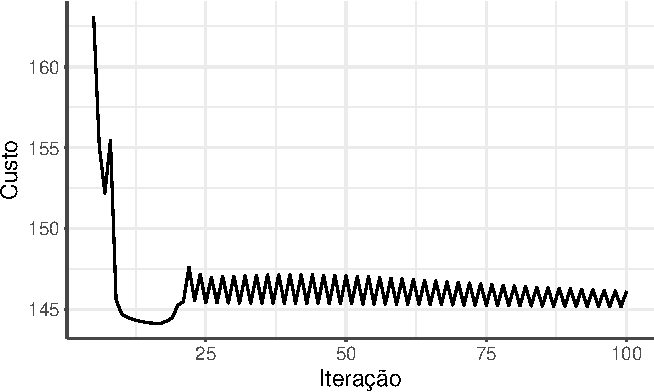
\includegraphics{lista1-resolucao_files/figure-pdf/fig-historico-custo-1.pdf}

}

\caption{\label{fig-historico-custo}Histórico de custo para o banco de
validação.}

\end{figure}%

O vetor de pesos estimado para a iteração de menor valor da perda foi:

\begin{align*}
\hat{W}^{(1)} = \begin{pmatrix} -1.6958498 & -1.6958498 \\ -2.6882879 & -2.6882879 \end{pmatrix}, \quad 
%
\hat{\boldsymbol{b}}^{(1)} = \begin{pmatrix} 3.4379156 \\ 3.4379156 \end{pmatrix},
\end{align*}

\begin{align*}
\hat{W}^{(2)} = \begin{pmatrix} 8.7439654 \\ 8.7439654 \end{pmatrix}, \quad 
%
\hat{\boldsymbol{b}}^{(2)} = 9.7284693.
\end{align*}

Interessantemente, os pesos de cada variavel para a camada seguinte,
assim como os viéses, são idênticos. Além disso, os pesos aplicados nos
neurônios da camada escondida também são idênticos. Isso pode ser um
indicativo de que ambas as variáveis explicativas possuem importância
igual para a previsão da variável resposta. Ao mesmo tempo, ambas
\(X_1\) e \(X_2\) têm o mesmo processo gerador, então não parece ser
surpreendente que os pesos sejam iguais.

Finalmente, o gráfico indica que possivelmente o algoritmo estacionou em
um mínimo local de valor superior ao mínimo encontrado na iteração de
número 16.

\subsection{Item f}\label{item-f}

Apresente o gráfico do custo no conjunto de treinamento e no de
validação (uma linha para cada) em função do número da interação do
processo de otimização. Comente os resultados.

\begin{center}\rule{0.5\linewidth}{0.5pt}\end{center}

A seguir é construido o gráfico. Novamemente, trata-se de duas bases de
dados relativamente simples, com um mesmo processo gerador dos dados e
uma quantidade razoável de pontos, então é esperado que o custo de
treinamento e validação sejam semelhantes.

Apesar disso, é possível notar que, na base de treinamento, o algoritmo
escapa do mínimo identificado ligeiramente mais rápido, possivelmente
devido à maior disponibilidade de dados. Neste caso, a base de
treinamento é oito vezes maior que a base de validação.

\begin{Shaded}
\begin{Highlighting}[]
\CommentTok{\# hiperparametros e base de treinamento}
\NormalTok{learning\_rate }\OtherTok{\textless{}{-}}  \FloatTok{0.1}
\NormalTok{epochs }\OtherTok{\textless{}{-}} \DecValTok{100}\NormalTok{L}
\NormalTok{y }\OtherTok{\textless{}{-}}\NormalTok{ dados\_train}\SpecialCharTok{$}\NormalTok{y}
\NormalTok{x }\OtherTok{\textless{}{-}}\NormalTok{ dados\_train[,}\FunctionTok{c}\NormalTok{(}\DecValTok{1}\NormalTok{,}\DecValTok{2}\NormalTok{)]}

\NormalTok{comparacao\_treino\_validacao }\OtherTok{\textless{}{-}} \FunctionTok{tibble}\NormalTok{(}
  \AttributeTok{epoch =} \FunctionTok{rep}\NormalTok{(}\DecValTok{1}\SpecialCharTok{:}\NormalTok{epochs, }\DecValTok{2}\NormalTok{),}
  \AttributeTok{base =} \FunctionTok{rep}\NormalTok{(}\FunctionTok{c}\NormalTok{(}\StringTok{"Validação"}\NormalTok{, }\StringTok{"Treinamento"}\NormalTok{), }\AttributeTok{each =}\NormalTok{ epochs),}
  \CommentTok{\# back\_validacao foi gerada no item e}
  \AttributeTok{loss =} \FunctionTok{c}\NormalTok{(back\_validacao}\SpecialCharTok{$}\NormalTok{loss\_history, }\FunctionTok{backpropagation}\NormalTok{(x, theta, y, learning\_rate, epochs)}\SpecialCharTok{$}\NormalTok{loss\_history)}
\NormalTok{)}

\NormalTok{comparacao\_treino\_validacao }\SpecialCharTok{\%\textgreater{}\%}
  \FunctionTok{filter}\NormalTok{(loss }\SpecialCharTok{\textless{}} \DecValTok{170}\NormalTok{) }\SpecialCharTok{\%\textgreater{}\%}
  \FunctionTok{ggplot}\NormalTok{(}\FunctionTok{aes}\NormalTok{(epoch, loss, }\AttributeTok{group =}\NormalTok{ base, }\AttributeTok{color =}\NormalTok{ base))}\SpecialCharTok{+}
  \FunctionTok{geom\_line}\NormalTok{(}\AttributeTok{alpha =}\NormalTok{ .}\DecValTok{5}\NormalTok{)}\SpecialCharTok{+}
  \FunctionTok{labs}\NormalTok{(}\AttributeTok{x =} \StringTok{"Iteração"}\NormalTok{,}
       \AttributeTok{y =} \StringTok{"Custo"}\NormalTok{,}
       \AttributeTok{color =} \StringTok{""}\NormalTok{)}\SpecialCharTok{+}
  \FunctionTok{theme\_bw}\NormalTok{()}\SpecialCharTok{+}
    \FunctionTok{theme}\NormalTok{(}\AttributeTok{panel.border =} \FunctionTok{element\_blank}\NormalTok{(), }\CommentTok{\# Remove all panel borders}
        \AttributeTok{axis.line =} \FunctionTok{element\_line}\NormalTok{(}\AttributeTok{color =} \StringTok{"\#474747"}\NormalTok{), }\CommentTok{\# Add axis lines}
        \AttributeTok{axis.ticks.x =} \FunctionTok{element\_line}\NormalTok{(}\AttributeTok{color =} \StringTok{"\#474747"}\NormalTok{), }\CommentTok{\# X axis ticks}
        \AttributeTok{axis.ticks.y =} \FunctionTok{element\_line}\NormalTok{(}\AttributeTok{color =} \StringTok{"\#474747"}\NormalTok{), }\CommentTok{\# Y axis ticks}
        \AttributeTok{axis.ticks.length =} \FunctionTok{unit}\NormalTok{(}\FloatTok{0.05}\NormalTok{, }\StringTok{"cm"}\NormalTok{), }\CommentTok{\# Control tick length}
        \AttributeTok{legend.position =} \StringTok{"bottom"}\NormalTok{) }
\end{Highlighting}
\end{Shaded}

\begin{figure}[H]

\centering{

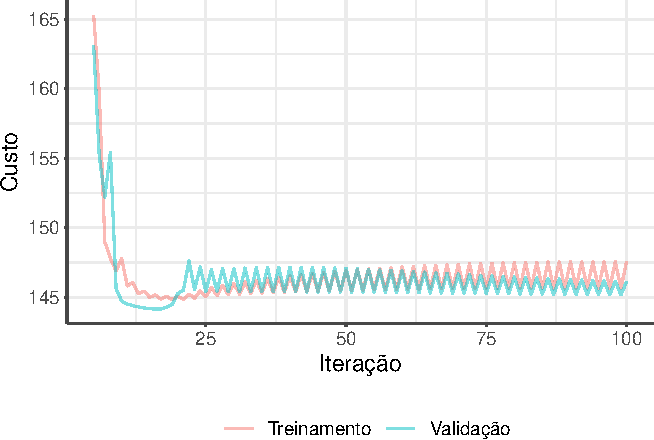
\includegraphics{lista1-resolucao_files/figure-pdf/fig-historico-custo-treinamento-validacao-1.pdf}

}

\caption{\label{fig-historico-custo-treinamento-validacao}Histórico de
custo para o banco de treinamento e validação.}

\end{figure}%

\subsection{Item g}\label{item-g}

Calcule os valores previstos \((\hat{y}_i)\) e os resíduos
\((y_i - \hat{y}_i)\) da rede no conjunto de teste e represente-os
graficamente em função de \(x_1\) e \(x_2\). Dica: tome como base o
código usado para a visualização da superfície
\((E(Y |X_1, X_2), X_1, X_2)\). Altere o gradiente de cores e, se
necessário, use pontos semi-transparentes. Analise o desempenho da rede
nas diferentes regiões do plano. Há locais onde o modelo é claramente
viesado ou menos acurado?

\begin{center}\rule{0.5\linewidth}{0.5pt}\end{center}

\begin{Shaded}
\begin{Highlighting}[]
\CommentTok{\#calcular o back propagation e usar o melhor theta do conjunto de teste}

\CommentTok{\# usamos o conjunto de teste}
\NormalTok{theta }\OtherTok{\textless{}{-}}\NormalTok{ back\_validacao}\SpecialCharTok{$}\NormalTok{theta}

\NormalTok{resultados\_gradiente }\OtherTok{\textless{}{-}} \FunctionTok{gradiente}\NormalTok{(dados\_test[,}\FunctionTok{c}\NormalTok{(}\DecValTok{1}\NormalTok{,}\DecValTok{2}\NormalTok{)], theta, dados\_test}\SpecialCharTok{$}\NormalTok{y)}

\NormalTok{residuos }\OtherTok{=}\NormalTok{ resultados\_gradiente}\SpecialCharTok{$}\NormalTok{loss\_results}\SpecialCharTok{$}\NormalTok{diff}

\CommentTok{\# usamos o conjunto de teste}
\NormalTok{dados\_graf\_residuos }\OtherTok{\textless{}{-}}\NormalTok{ dados\_test }\SpecialCharTok{\%\textgreater{}\%}
  \FunctionTok{select}\NormalTok{(x1.obs, x2.obs, y) }\SpecialCharTok{\%\textgreater{}\%} \CommentTok{\#seleciona variaveis de interesse}
  \FunctionTok{mutate}\NormalTok{(}\AttributeTok{residuos =}\NormalTok{ residuos,}
         \AttributeTok{yhat =}\NormalTok{ resultados\_gradiente}\SpecialCharTok{$}\NormalTok{loss\_results}\SpecialCharTok{$}\NormalTok{yhat}
\NormalTok{         )}

\CommentTok{\# base do gráfico}
\NormalTok{plot\_residuos }\OtherTok{\textless{}{-}} \FunctionTok{ggplot}\NormalTok{(dados\_graf\_residuos, }\FunctionTok{aes}\NormalTok{(}\AttributeTok{x=}\NormalTok{x1.obs, }\AttributeTok{y=}\NormalTok{x2.obs)) }\SpecialCharTok{+}
  \FunctionTok{geom\_point}\NormalTok{(}\FunctionTok{aes}\NormalTok{(}\AttributeTok{colour=}\NormalTok{residuos), }\AttributeTok{size=}\DecValTok{2}\NormalTok{, }\AttributeTok{shape=}\DecValTok{15}\NormalTok{, }\AttributeTok{alpha =}\NormalTok{ .}\DecValTok{3}\NormalTok{) }\SpecialCharTok{+}
  \FunctionTok{coord\_cartesian}\NormalTok{(}\AttributeTok{expand=}\NormalTok{F) }\SpecialCharTok{+}
  \FunctionTok{scale\_colour\_gradient}\NormalTok{(}\AttributeTok{low=}\StringTok{"white"}\NormalTok{,}
    \AttributeTok{high=}\StringTok{"black"}\NormalTok{,}
    \AttributeTok{name=}\StringTok{"Resíduos"}\NormalTok{) }\SpecialCharTok{+}
  \FunctionTok{xlab}\NormalTok{(}\FunctionTok{TeX}\NormalTok{(}\StringTok{"$X\_1$"}\NormalTok{)) }\SpecialCharTok{+} \FunctionTok{ylab}\NormalTok{(}\FunctionTok{TeX}\NormalTok{(}\StringTok{"$X\_2$"}\NormalTok{))}\SpecialCharTok{+}
  \FunctionTok{theme}\NormalTok{(}\AttributeTok{legend.position =} \StringTok{"bottom"}\NormalTok{,}
        \AttributeTok{axis.title.y =} \FunctionTok{element\_text}\NormalTok{(}\AttributeTok{angle =} \DecValTok{0}\NormalTok{, }\AttributeTok{vjust =} \FloatTok{0.5}\NormalTok{))}

\CommentTok{\#gráfico da esperança}
\NormalTok{n }\OtherTok{\textless{}{-}} \DecValTok{100}
\NormalTok{x1 }\OtherTok{\textless{}{-}} \FunctionTok{seq}\NormalTok{(}\SpecialCharTok{{-}}\DecValTok{3}\NormalTok{, }\DecValTok{3}\NormalTok{, }\AttributeTok{length.out=}\NormalTok{n)}
\NormalTok{x2 }\OtherTok{\textless{}{-}} \FunctionTok{seq}\NormalTok{(}\SpecialCharTok{{-}}\DecValTok{3}\NormalTok{, }\DecValTok{3}\NormalTok{, }\AttributeTok{length.out=}\NormalTok{n)}
\NormalTok{dados.grid }\OtherTok{\textless{}{-}} \FunctionTok{as\_tibble}\NormalTok{(}\FunctionTok{expand.grid}\NormalTok{(x1, x2)) }\SpecialCharTok{\%\textgreater{}\%}
  \FunctionTok{rename\_all}\NormalTok{(}\SpecialCharTok{\textasciitilde{}} \FunctionTok{c}\NormalTok{(}\StringTok{"x1"}\NormalTok{, }\StringTok{"x2"}\NormalTok{)) }\SpecialCharTok{\%\textgreater{}\%}
  \FunctionTok{mutate}\NormalTok{(}\AttributeTok{mu=}\FunctionTok{abs}\NormalTok{(x1}\SpecialCharTok{\^{}}\DecValTok{3} \SpecialCharTok{{-}} \DecValTok{30}\SpecialCharTok{*}\FunctionTok{sin}\NormalTok{(x2) }\SpecialCharTok{+} \DecValTok{10}\NormalTok{))}

\NormalTok{plot\_esperanca }\OtherTok{\textless{}{-}} \FunctionTok{ggplot}\NormalTok{(dados.grid, }\FunctionTok{aes}\NormalTok{(}\AttributeTok{x=}\NormalTok{x1, }\AttributeTok{y=}\NormalTok{x2)) }\SpecialCharTok{+}
  \FunctionTok{geom\_point}\NormalTok{(}\FunctionTok{aes}\NormalTok{(}\AttributeTok{colour=}\NormalTok{mu), }\AttributeTok{size=}\DecValTok{2}\NormalTok{, }\AttributeTok{shape=}\DecValTok{15}\NormalTok{) }\SpecialCharTok{+}
  \FunctionTok{coord\_cartesian}\NormalTok{(}\AttributeTok{expand=}\NormalTok{F) }\SpecialCharTok{+}
  \FunctionTok{scale\_colour\_gradient}\NormalTok{(}\AttributeTok{low=}\StringTok{"white"}\NormalTok{,}
  \AttributeTok{high=}\StringTok{"black"}\NormalTok{,}
  \AttributeTok{name=}\FunctionTok{TeX}\NormalTok{(}\StringTok{"$E(Y|X\_1, X\_2)$"}\NormalTok{)) }\SpecialCharTok{+}
  \FunctionTok{xlab}\NormalTok{(}\FunctionTok{TeX}\NormalTok{(}\StringTok{"$X\_1$"}\NormalTok{)) }\SpecialCharTok{+} \FunctionTok{ylab}\NormalTok{(}\FunctionTok{TeX}\NormalTok{(}\StringTok{"$X\_2$"}\NormalTok{))}\SpecialCharTok{+}
  \FunctionTok{theme}\NormalTok{(}\AttributeTok{legend.position =} \StringTok{"bottom"}\NormalTok{,}
        \AttributeTok{axis.title.y =} \FunctionTok{element\_text}\NormalTok{(}\AttributeTok{angle =} \DecValTok{0}\NormalTok{, }\AttributeTok{vjust =} \FloatTok{0.5}\NormalTok{))}
\end{Highlighting}
\end{Shaded}

O gráfico dos resíduos utilizando o gradiente implementado e o gráfico
da esperança são apresentados a seguir. Interessantemente, o resíduo
parece ser parece ser maior em regiões em que a esperança
\(E(Y |X_1, X_2)\) é maior e menor onde a esperança é menor. A região de
resíduos próximos a zero é uma região intermediária que margeia o
senóide.

\begin{Shaded}
\begin{Highlighting}[]
\FunctionTok{plot\_grid}\NormalTok{(plot\_residuos, plot\_esperanca, }\AttributeTok{ncol=}\DecValTok{2}\NormalTok{)}
\end{Highlighting}
\end{Shaded}

\begin{figure}[H]

\centering{

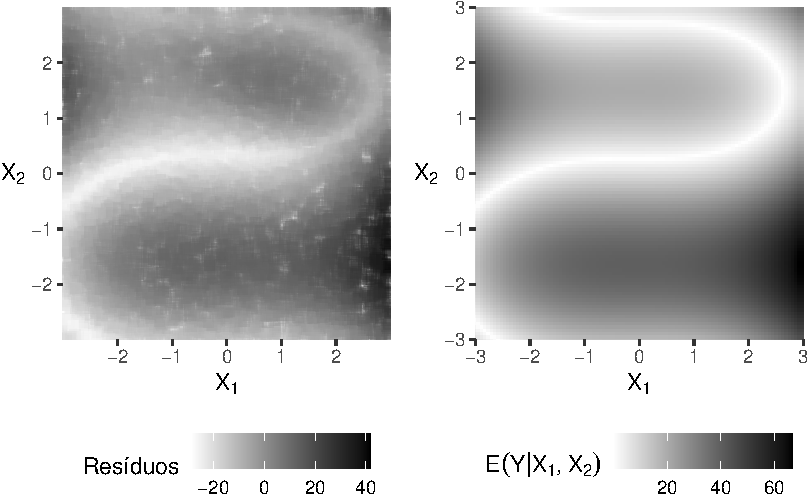
\includegraphics{lista1-resolucao_files/figure-pdf/fig-predicao-residuos-1.pdf}

}

\caption{\label{fig-predicao-residuos}Resíduos da rede em função de
\(X_1\) e \(X_2\).}

\end{figure}%

\subsection{Item h}\label{item-h}

Faça um gráfico do valor observado \(y_i\) em função do valor esperado
\(\hat{y}_i = E(Y_i |x_{1i} , x_{2i})\) para cada observação do conjunto
de teste. Interprete o resultado.

\begin{center}\rule{0.5\linewidth}{0.5pt}\end{center}

No gráfico abaixo é possível observar que os valores de \(\hat{y}\)
tendem a se concentrar nas extremidades e parece haver uma sobreposição
de comportamentos na transição entre os valores extremos do valor
esperado.

Enquanto parece haver uma grande dispersão em toda a região observada,
os valores entre os extremos de \(\hat{y}\) parecem ter menor variância
e estão mais concentrados em torno do valor esperado --- apesar de haver
pontos bem distantes. Além disso, fica evidente a maior variância para
para valores extremos de \(\hat{y}\).

\begin{Shaded}
\begin{Highlighting}[]
\NormalTok{dados\_graf\_residuos }\SpecialCharTok{\%\textgreater{}\%}
  \FunctionTok{ggplot}\NormalTok{(}\FunctionTok{aes}\NormalTok{(yhat, y))}\SpecialCharTok{+}
  \FunctionTok{geom\_point}\NormalTok{(}\AttributeTok{alpha =} \FloatTok{0.3}\NormalTok{)}\SpecialCharTok{+}
  \FunctionTok{geom\_abline}\NormalTok{(}\AttributeTok{slope =} \DecValTok{1}\NormalTok{, }\AttributeTok{intercept =} \DecValTok{0}\NormalTok{, }\AttributeTok{color =} \StringTok{"red"}\NormalTok{)}\SpecialCharTok{+}
  \FunctionTok{theme\_bw}\NormalTok{()}\SpecialCharTok{+}
  \FunctionTok{labs}\NormalTok{(}\AttributeTok{x =} \FunctionTok{TeX}\NormalTok{(}\StringTok{"$}\SpecialCharTok{\textbackslash{}\textbackslash{}}\StringTok{hat\{y\}\_i$"}\NormalTok{), }\AttributeTok{y =} \FunctionTok{TeX}\NormalTok{(}\StringTok{"$y\_i$"}\NormalTok{))}\SpecialCharTok{+}
  \FunctionTok{theme}\NormalTok{(}\AttributeTok{panel.border =} \FunctionTok{element\_blank}\NormalTok{(), }\CommentTok{\# Remove all panel borders}
    \AttributeTok{axis.line =} \FunctionTok{element\_line}\NormalTok{(}\AttributeTok{color =} \StringTok{"\#474747"}\NormalTok{), }\CommentTok{\# Add axis lines}
    \AttributeTok{axis.ticks.x =} \FunctionTok{element\_line}\NormalTok{(}\AttributeTok{color =} \StringTok{"\#474747"}\NormalTok{), }\CommentTok{\# X axis ticks}
    \AttributeTok{axis.ticks.y =} \FunctionTok{element\_line}\NormalTok{(}\AttributeTok{color =} \StringTok{"\#474747"}\NormalTok{), }\CommentTok{\# Y axis ticks}
    \AttributeTok{axis.ticks.length =} \FunctionTok{unit}\NormalTok{(}\FloatTok{0.05}\NormalTok{, }\StringTok{"cm"}\NormalTok{), }\CommentTok{\# Control tick length}
    \AttributeTok{legend.position =} \StringTok{"bottom"}\NormalTok{,}
    \AttributeTok{axis.title.y =} \FunctionTok{element\_text}\NormalTok{(}\AttributeTok{angle =} \DecValTok{0}\NormalTok{, }\AttributeTok{vjust =} \FloatTok{0.5}\NormalTok{)) }
\end{Highlighting}
\end{Shaded}

\begin{figure}[H]

\centering{

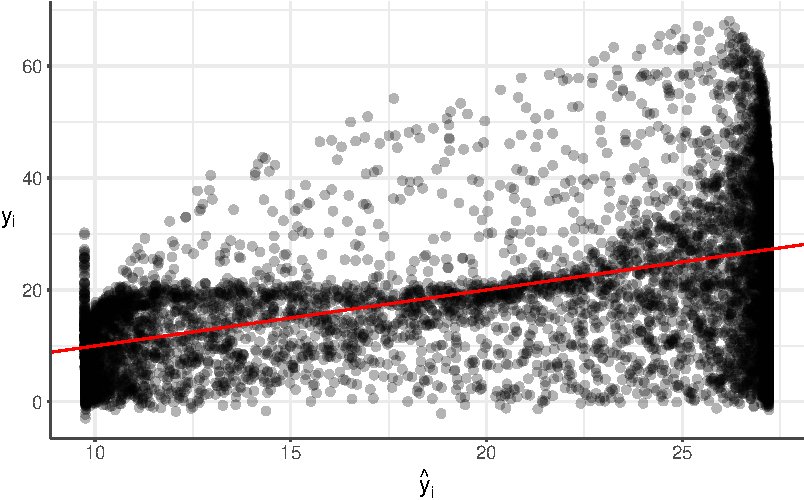
\includegraphics{lista1-resolucao_files/figure-pdf/fig-esperadoobservado-1.pdf}

}

\caption{\label{fig-esperadoobservado}Valor observado em função do valor
esperado gerado pela rede neural.}

\end{figure}%

\subsection{Item i}\label{item-i}

Para cada \(k = 1,\dots, 300\), recalcule o gradiente obtido no item d)
usando apenas as \(k\)-primeiras observações do banco de dados original.
Novamente, use \(\boldsymbol{\theta} = (0.1, \dots, 0.1)\). Apresente um
gráfico com o valor do primeiro elemento do gradiente --- isso é, a
derivada parcial \(\frac{\partial J}{\partial w_1}\) --- em função do
número de amostras \(k\). Como referência, adicione uma linha horizontal
vermelha indicando o valor obtido em d). Em seguida, use a função
\texttt{microbenchmark} para comparar o tempo de cálculo do gradiente
para \(k = 300\) e \(k = 100000\). Explique de que maneira os resultados
dessa análise podem ser usados para acelerar a execução do item e).

\begin{center}\rule{0.5\linewidth}{0.5pt}\end{center}

Primeiro são obtidos os elementos \(\frac{\partial J}{\partial w_1}\)
para as amostras de tamanho 1 a 300:

\begin{Shaded}
\begin{Highlighting}[]
\NormalTok{theta }\OtherTok{\textless{}{-}} \FunctionTok{list}\NormalTok{(}
  \AttributeTok{M1 =} \FunctionTok{matrix}\NormalTok{(}\FunctionTok{c}\NormalTok{(}\FloatTok{0.1}\NormalTok{), }\AttributeTok{nrow =} \DecValTok{2}\NormalTok{, }\AttributeTok{ncol =} \DecValTok{2}\NormalTok{), }
  \AttributeTok{b12 =} \FunctionTok{c}\NormalTok{(}\FloatTok{0.1}\NormalTok{, }\FloatTok{0.1}\NormalTok{), }
  \AttributeTok{M2 =} \FunctionTok{matrix}\NormalTok{(}\FunctionTok{c}\NormalTok{(}\FloatTok{0.1}\NormalTok{), }\AttributeTok{nrow =} \DecValTok{2}\NormalTok{, }\AttributeTok{ncol =} \DecValTok{1}\NormalTok{), }
  \AttributeTok{b3 =} \FunctionTok{c}\NormalTok{(}\FloatTok{0.1}\NormalTok{) }
\NormalTok{)}

\NormalTok{k\_w1 }\OtherTok{\textless{}{-}} \ControlFlowTok{function}\NormalTok{(dados, theta, i)\{}
\NormalTok{  base }\OtherTok{\textless{}{-}}\NormalTok{ dados[}\DecValTok{1}\SpecialCharTok{:}\NormalTok{i,}\FunctionTok{c}\NormalTok{(}\DecValTok{1}\NormalTok{, }\DecValTok{2}\NormalTok{)] }\CommentTok{\#dados com linha 1 ate i}
\NormalTok{  y }\OtherTok{\textless{}{-}}\NormalTok{ dados}\SpecialCharTok{$}\NormalTok{y[}\DecValTok{1}\SpecialCharTok{:}\NormalTok{i] }\CommentTok{\#target com linhas 1 até i}
  \FunctionTok{return}\NormalTok{(}\FunctionTok{gradiente}\NormalTok{(base, theta, y)}\SpecialCharTok{$}\NormalTok{grad[}\DecValTok{1}\NormalTok{]) }\CommentTok{\#retorna w1}
\NormalTok{\}}

\NormalTok{valores\_w1 }\OtherTok{\textless{}{-}} \FunctionTok{tibble}\NormalTok{(}
  \AttributeTok{k =} \DecValTok{1}\SpecialCharTok{:}\DecValTok{300}\NormalTok{,}
  \AttributeTok{w1 =} \FunctionTok{map\_dbl}\NormalTok{(k, }\SpecialCharTok{\textasciitilde{}} \FunctionTok{k\_w1}\NormalTok{(dados, theta, .))}
\NormalTok{)}
\end{Highlighting}
\end{Shaded}

O gráfico do valor de \(w_1\) calculado em função do tamanho da amostra
é exibido a seguir. Como é de se esperar, o valor de \(w_1\) tende a se
aproximar do valor obtido no item d) à medida que o tamanho da amostra
aumenta.

\begin{Shaded}
\begin{Highlighting}[]
\FunctionTok{ggplot}\NormalTok{(valores\_w1, }\FunctionTok{aes}\NormalTok{(k, w1, }\AttributeTok{group =} \DecValTok{1}\NormalTok{))}\SpecialCharTok{+}
  \FunctionTok{geom\_line}\NormalTok{()}\SpecialCharTok{+}
  \FunctionTok{geom\_hline}\NormalTok{(}\AttributeTok{yintercept =}\NormalTok{ grad\_item\_d[}\StringTok{"w1"}\NormalTok{], }\AttributeTok{color =} \StringTok{"red"}\NormalTok{)}\SpecialCharTok{+}
  \FunctionTok{theme\_bw}\NormalTok{()}\SpecialCharTok{+}
  \FunctionTok{labs}\NormalTok{(}\AttributeTok{x =} \StringTok{"Tamanho da amostra"}\NormalTok{, }\AttributeTok{y =} \FunctionTok{TeX}\NormalTok{(}\StringTok{"$w\_1$"}\NormalTok{))}\SpecialCharTok{+}
  \FunctionTok{theme}\NormalTok{(}\AttributeTok{panel.border =} \FunctionTok{element\_blank}\NormalTok{(), }\CommentTok{\# Remove all panel borders}
    \AttributeTok{axis.line =} \FunctionTok{element\_line}\NormalTok{(}\AttributeTok{color =} \StringTok{"\#474747"}\NormalTok{), }\CommentTok{\# Add axis lines}
    \AttributeTok{axis.ticks.x =} \FunctionTok{element\_line}\NormalTok{(}\AttributeTok{color =} \StringTok{"\#474747"}\NormalTok{), }\CommentTok{\# X axis ticks}
    \AttributeTok{axis.ticks.y =} \FunctionTok{element\_line}\NormalTok{(}\AttributeTok{color =} \StringTok{"\#474747"}\NormalTok{), }\CommentTok{\# Y axis ticks}
    \AttributeTok{axis.ticks.length =} \FunctionTok{unit}\NormalTok{(}\FloatTok{0.05}\NormalTok{, }\StringTok{"cm"}\NormalTok{), }\CommentTok{\# Control tick length}
    \AttributeTok{legend.position =} \StringTok{"bottom"}\NormalTok{,}
    \AttributeTok{axis.title.y =} \FunctionTok{element\_text}\NormalTok{(}\AttributeTok{angle =} \DecValTok{0}\NormalTok{, }\AttributeTok{vjust =} \FloatTok{0.5}\NormalTok{))}\SpecialCharTok{+}
    \FunctionTok{annotate}\NormalTok{(}\StringTok{"text"}\NormalTok{, }\AttributeTok{x =} \DecValTok{200}\NormalTok{, }\AttributeTok{y =} \DecValTok{0}\NormalTok{, }
           \AttributeTok{label =} \FunctionTok{paste0}\NormalTok{(}\StringTok{"w1 = "}\NormalTok{,}\FunctionTok{round}\NormalTok{(grad\_item\_d[}\StringTok{"w1"}\NormalTok{],}\DecValTok{2}\NormalTok{)), }
           \AttributeTok{hjust =} \DecValTok{1}\NormalTok{, }\AttributeTok{vjust =} \DecValTok{0}\NormalTok{, }\AttributeTok{size =} \DecValTok{4}\NormalTok{, }\AttributeTok{color =} \StringTok{"red"}\NormalTok{)}
\end{Highlighting}
\end{Shaded}

\begin{figure}[H]

\centering{

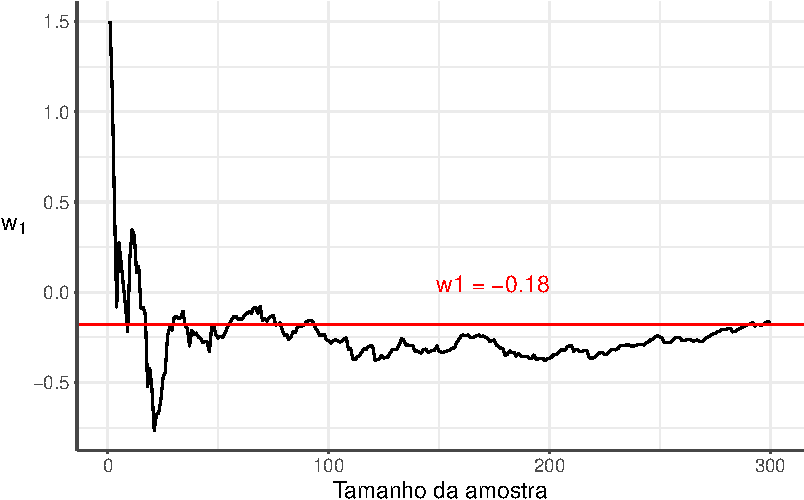
\includegraphics{lista1-resolucao_files/figure-pdf/fig-gradientek-1.pdf}

}

\caption{\label{fig-gradientek}Valor do gradiente
\(\frac{\partial J}{\partial w_1}\) em função do tamanho da amostra.}

\end{figure}%

~

Nota-se do gráfico na Figura~\ref{fig-gradientek} que o valor de \(w_1\)
tende a se aproximar do valor obtido no item d) à medida que o tamanho
da amostra aumenta. Ao mesmo tempo, o resultado do benchmark exposto na
Tabela~\ref{tbl-microbenchmark} sugere um tempo muito menor para o
cálculo do gradiente com amostras menores. Se com uma amostra de tamanho
300 o tempo médio de execução tem uma diferença de duas ordens de
grandeza em relação à amostra de tamanho 100.000 e o resultado para o
gradiente é muito próximo, uma possibilidade para acelerar ainda mais a
execução do item e) seria realizar o cálculo do gradiente em pacotes
(\emph{batches}).

\begin{Shaded}
\begin{Highlighting}[]
\NormalTok{microbenchmark}\SpecialCharTok{::}\FunctionTok{microbenchmark}\NormalTok{(}
  \AttributeTok{k\_300 =} \FunctionTok{k\_w1}\NormalTok{(dados, theta, }\DecValTok{300}\NormalTok{),}
  \AttributeTok{k\_100000 =} \FunctionTok{k\_w1}\NormalTok{(dados, theta, }\DecValTok{100000}\NormalTok{),}
  \AttributeTok{times =} \DecValTok{100}
\NormalTok{) }\SpecialCharTok{\%\textgreater{}\%}
  \FunctionTok{summary}\NormalTok{() }\SpecialCharTok{\%\textgreater{}\%}
  \FunctionTok{select}\NormalTok{(}\SpecialCharTok{{-}}\NormalTok{neval) }\SpecialCharTok{\%\textgreater{}\%}
\NormalTok{  knitr}\SpecialCharTok{::}\FunctionTok{kable}\NormalTok{(}\AttributeTok{digits =} \DecValTok{2}\NormalTok{)}
\end{Highlighting}
\end{Shaded}

\begin{longtable}[]{@{}lrrrrrr@{}}

\caption{\label{tbl-microbenchmark}Resultados do microbenchmark para o
cálculo do gradiente com k = 300 e k = 100.000.}

\tabularnewline

\toprule\noalign{}
expr & min & lq & mean & median & uq & max \\
\midrule\noalign{}
\endhead
\bottomrule\noalign{}
\endlastfoot
k\_300 & 300.42 & 335.80 & 2506.44 & 468.45 & 605.81 & 184091.3 \\
k\_100000 & 24486.86 & 32429.66 & 44916.49 & 33818.33 & 36363.58 &
226434.2 \\

\end{longtable}

~

\subsection{Item j}\label{item-j}

Ajuste sobre o conjunto de treinamento um modelo linear normal (modelo
linear 1) \[
Y_i = N \left(\beta_0 + \beta_1 x_{1i} + \beta_2 x_{2i}, \sigma \right)
\]

usando a função \texttt{lm} do pacote \texttt{R} (ou outra equivalente).
Em seguida, inclua na lista de covariáveis termos quadráticos e de
interação linear. Isso é, assuma que no modelo linear 2,

\[
E(Y|x_1, x_2) = \beta_0 + \beta_1 x_{1} + \beta_2 x_{2} + \beta_3 x_1^2 + \beta_4 x_2^2 + \beta_5 x_1 x_2.
\]

Compare o erro quadrático médio no conjunto de teste dos dois modelos
lineares acima com o da rede neural ajustada anteriormente. Qual dos 3
modelos você usaria para previsão? Justifique sua resposta.

\begin{center}\rule{0.5\linewidth}{0.5pt}\end{center}

Os modelos lineares são ajustados a seguir:

\begin{Shaded}
\begin{Highlighting}[]
\NormalTok{MSE1 }\OtherTok{\textless{}{-}} \FunctionTok{lm}\NormalTok{(y }\SpecialCharTok{\textasciitilde{}}\NormalTok{ x1.obs }\SpecialCharTok{+}\NormalTok{ x2.obs, }\AttributeTok{data =}\NormalTok{ dados\_train) }\SpecialCharTok{\%\textgreater{}\%}
  \FunctionTok{anova}\NormalTok{() }\SpecialCharTok{\%\textgreater{}\%} 
  \FunctionTok{pull}\NormalTok{(}\StringTok{\textasciigrave{}}\AttributeTok{Mean Sq}\StringTok{\textasciigrave{}}\NormalTok{) }\SpecialCharTok{\%\textgreater{}\%}
  \FunctionTok{min}\NormalTok{()}

\NormalTok{MSE2 }\OtherTok{\textless{}{-}} \FunctionTok{lm}\NormalTok{(y }\SpecialCharTok{\textasciitilde{}}\NormalTok{ x1.obs}\SpecialCharTok{*}\NormalTok{x2.obs }\SpecialCharTok{+} \FunctionTok{I}\NormalTok{(x1.obs}\SpecialCharTok{\^{}}\DecValTok{2}\NormalTok{) }\SpecialCharTok{+} \FunctionTok{I}\NormalTok{(x2.obs}\SpecialCharTok{\^{}}\DecValTok{2}\NormalTok{), }\AttributeTok{data =}\NormalTok{ dados\_train) }\SpecialCharTok{\%\textgreater{}\%}
  \FunctionTok{anova}\NormalTok{() }\SpecialCharTok{\%\textgreater{}\%} 
  \FunctionTok{pull}\NormalTok{(}\StringTok{\textasciigrave{}}\AttributeTok{Mean Sq}\StringTok{\textasciigrave{}}\NormalTok{) }\SpecialCharTok{\%\textgreater{}\%}
  \FunctionTok{min}\NormalTok{()}

\NormalTok{MSErn }\OtherTok{\textless{}{-}} \FunctionTok{min}\NormalTok{(back\_validacao}\SpecialCharTok{$}\NormalTok{loss\_history)}
\end{Highlighting}
\end{Shaded}

As perdas quadráticas são expostas na tabela a seguir:

\begin{longtable}[]{@{}lr@{}}

\caption{\label{tbl-MSE}Perdas quadráticas dos modelos ajustados.}

\tabularnewline

\toprule\noalign{}
Modelo & MSE \\
\midrule\noalign{}
\endhead
\bottomrule\noalign{}
\endlastfoot
Rede Neural & 144.15 \\
Modelo Linear 1 & 138.71 \\
Modelo Linear 2 & 94.76 \\

\end{longtable}

Pautado exclusivamente pelas perdas quadráticas, o modelo que deveria
ser escolhido deveria ser o Modelo Linear 2, que inclui interações e
termos quadráticos. No entanto, é importante considerar também a
capacidade de generalização do modelo. Uma avaliação desses modelos
considerando outras bases de dados para teste seria necessária para
determinar o melhor desempenho.

\subsection{Item k}\label{item-k}

Para cada modelo ajustado (os dois lineares e a rede neural), descreva o
efeito no valor esperado da variável resposta causado por um aumento de
uma unidade da covariável \(x_1\)?

\begin{center}\rule{0.5\linewidth}{0.5pt}\end{center}

Temos como variação no valor esperado da variável resposta em função do
incremento unitário de \(x_1\) as expressões e valores a seguir:

\textbf{Modelo 1}

\(\frac{d \, \hat{y}}{d \, x_1} = \hat{\beta}_1 =\) 1.2 ~

\textbf{Modelo 2}

\(\frac{d \, \hat{y}}{d \, x_1} = \hat{\beta}_1 + 2\hat{\beta}_3 \, x_1 + \hat{\beta}_5 x_2 =\)
1.19 + 1.4\(x_1\) + -2.09555 \(x_2\) ~

\textbf{Rede Neural}

\(\frac{\partial \, \hat{y}_i}{\partial \, x_{1i}} = w_5 \, \frac{\partial}{\partial x_{1i}} h_{1i} + w_6\, \frac{\partial}{\partial x_{1i}} h_{2i} = w_5w_1 \, \frac{e^{-a_{1i}}}{(1+e^{a_{1i}})^2} + w_6w_2 \, \frac{e^{-a_{2i}}}{(1+e^{a_{2i}})^2}\)

\subsection{Item l}\label{item-l}

Novamente, para cada um dos 3 modelos em estudo, calcule o percentual de
vezes que o intervalo de confiança de 95\% (para uma nova observação!)
capturou o valor de \(y_i\) . Considere apenas os dados do conjunto de
teste. No caso da rede neural, assuma que, aproximadamente,
\(\frac{y_i - \hat{y}_i}{\hat{\sigma}} \sim N (0, 1)\), onde
\(\hat{\sigma}\) representa a raiz do erro quadrático médio da rede.
Comente os resultados. Dica: para os modelos lineares, use a função
\texttt{predict(mod,\ interval="prediction")}.

\begin{center}\rule{0.5\linewidth}{0.5pt}\end{center}

Utilizamos os modelos gerados com a base de treinamento para fazer a
avaliação sobre os dados de teste.

\begin{Shaded}
\begin{Highlighting}[]
\CommentTok{\# modelo 1}
\NormalTok{predictm1 }\OtherTok{\textless{}{-}} \FunctionTok{predict}\NormalTok{(x1m1, }\AttributeTok{interval=}\StringTok{"prediction"}\NormalTok{, }\AttributeTok{newdata =}\NormalTok{ dados\_test) }\SpecialCharTok{\%\textgreater{}\%}
  \FunctionTok{tidy}\NormalTok{() }\SpecialCharTok{\%\textgreater{}\%}
  \FunctionTok{as.matrix}\NormalTok{(}\AttributeTok{ncol =} \DecValTok{3}\NormalTok{)}

\NormalTok{withinm1 }\OtherTok{\textless{}{-}}\NormalTok{ (dados\_test}\SpecialCharTok{$}\NormalTok{y }\SpecialCharTok{\textgreater{}=}\NormalTok{ predictm1[,}\DecValTok{2}\NormalTok{] }\SpecialCharTok{\&}\NormalTok{ dados\_test}\SpecialCharTok{$}\NormalTok{y }\SpecialCharTok{\textless{}=}\NormalTok{ predictm1[,}\DecValTok{3}\NormalTok{]) }\SpecialCharTok{\%\textgreater{}\%}
  \FunctionTok{mean}\NormalTok{()}

\CommentTok{\# modelo 2}
\NormalTok{predictm2 }\OtherTok{\textless{}{-}} \FunctionTok{predict}\NormalTok{(x1m2, }\AttributeTok{interval=}\StringTok{"prediction"}\NormalTok{, }\AttributeTok{data =}\NormalTok{ dados\_test) }\SpecialCharTok{\%\textgreater{}\%}
  \FunctionTok{tidy}\NormalTok{() }\SpecialCharTok{\%\textgreater{}\%}
  \FunctionTok{as.matrix}\NormalTok{(}\AttributeTok{ncol =} \DecValTok{3}\NormalTok{)}

\NormalTok{withinm2 }\OtherTok{\textless{}{-}}\NormalTok{ (dados\_test}\SpecialCharTok{$}\NormalTok{y }\SpecialCharTok{\textgreater{}=}\NormalTok{ predictm2[,}\DecValTok{2}\NormalTok{] }\SpecialCharTok{\&}\NormalTok{ dados\_test}\SpecialCharTok{$}\NormalTok{y }\SpecialCharTok{\textless{}=}\NormalTok{ predictm2[,}\DecValTok{3}\NormalTok{]) }\SpecialCharTok{\%\textgreater{}\%}
  \FunctionTok{mean}\NormalTok{()}

\CommentTok{\# rede neural}
\NormalTok{tabela\_withinrn }\OtherTok{\textless{}{-}} \FunctionTok{tibble}\NormalTok{(}
  \AttributeTok{yhat =} \FunctionTok{ffwd}\NormalTok{(dados\_test[,}\FunctionTok{c}\NormalTok{(}\DecValTok{1}\NormalTok{,}\DecValTok{2}\NormalTok{)], back\_validacao}\SpecialCharTok{$}\NormalTok{best\_theta)}\SpecialCharTok{$}\NormalTok{yhat,}
  \AttributeTok{sigma =} \FunctionTok{sqrt}\NormalTok{(}\FunctionTok{min}\NormalTok{(back\_validacao}\SpecialCharTok{$}\NormalTok{loss\_history)),}
  \AttributeTok{y =}\NormalTok{ dados\_test}\SpecialCharTok{$}\NormalTok{y,}
  \AttributeTok{std\_y =}\NormalTok{ (y}\SpecialCharTok{{-}}\NormalTok{yhat)}\SpecialCharTok{/}\NormalTok{sigma}
\NormalTok{) }\SpecialCharTok{\%\textgreater{}\%}
  \FunctionTok{mutate}\NormalTok{(}
    \AttributeTok{lower =}\NormalTok{ yhat }\SpecialCharTok{{-}} \FloatTok{1.96}\SpecialCharTok{*}\NormalTok{sigma,}
    \AttributeTok{upper =}\NormalTok{ yhat }\SpecialCharTok{+} \FloatTok{1.96}\SpecialCharTok{*}\NormalTok{sigma,}
    \AttributeTok{within =}\NormalTok{ (y }\SpecialCharTok{\textgreater{}=}\NormalTok{ lower }\SpecialCharTok{\&}\NormalTok{ y }\SpecialCharTok{\textless{}=}\NormalTok{ upper)}
\NormalTok{  )  }

\NormalTok{withinrn }\OtherTok{\textless{}{-}}\NormalTok{ tabela\_withinrn}\SpecialCharTok{\%\textgreater{}\%}
  \FunctionTok{pull}\NormalTok{(within) }\SpecialCharTok{\%\textgreater{}\%}
  \FunctionTok{mean}\NormalTok{()}
\end{Highlighting}
\end{Shaded}

As proporções dos valores de \(y_i\) que foram capturados pelos
intervalos de confiança gerados são exibidos na
Tabela~\ref{tbl-intervalos-confianca} a seguir. Enquanto o Modelo 2
obteve o menor MSE, a proporção dos valores reais capturados pelo
intervalo de confiança foi a menor entre os três modelos. Em comparação,
a rede neural apresentou o maior MSE, mas uma proporção de captura muito
similar ao Modelo Linear 1.

\begin{longtable}[]{@{}lrr@{}}

\caption{\label{tbl-intervalos-confianca}Proporção de valores de \(y_i\)
capturados pelos intervalos de confiança de 95\%.}

\tabularnewline

\toprule\noalign{}
Modelo & Proporção & MSE \\
\midrule\noalign{}
\endhead
\bottomrule\noalign{}
\endlastfoot
Modelo Linear 1 & 0.96 & 138.71 \\
Modelo Linear 2 & 0.74 & 94.76 \\
Rede Neural & 0.94 & 144.15 \\

\end{longtable}

\subsection{Item m}\label{item-m}

Para o modelo linear 1, faça um gráfico de dispersão entre \(x_1\) e
\(x_2\) onde cada ponto corresponde a uma observação do conjunto de
teste. Identifique os pontos que estavam contidos nos respectivos
intervalos de confiança utilizando a cor verde. Para os demais pontos,
use vermelho. Comente o resultado.

\begin{center}\rule{0.5\linewidth}{0.5pt}\end{center}

A seguir é construído o gráfico de dispersão conforme a instrução. Além
disso, o gráfico da esperança condicional de \(Y\) em função de \(X_1\)
e \(X_2\) é apresentado para comparação. Interessantemente os pontos
contidos nos intervalos de confiança parecem estar mais concentrados nas
regiões de maior valor da esperança condicional. No entanto, há pontos
no terceiro quadrante, que possuem baixos valores na esperança
condicional, que também não foram capturados --- esse padrão não se
repete em outros setores do gráfico. O padrão de não-captura (dentro do
domínio de \(X_1\) e \(X_2\) que estamos considerando) aparenta ser de
baixos valores de \(X_1\) com valoires extremos de \(X_2\) altos valores
de \(X_1\) dentro de um intervalo entre -1 e -2 para \(X_2\).

\begin{Shaded}
\begin{Highlighting}[]
\NormalTok{tabela }\OtherTok{\textless{}{-}} \FunctionTok{as\_tibble}\NormalTok{(predictm1) }\SpecialCharTok{\%\textgreater{}\%}
\NormalTok{  rlang}\SpecialCharTok{::}\FunctionTok{set\_names}\NormalTok{(}\StringTok{"yhat"}\NormalTok{,}\StringTok{"lower"}\NormalTok{, }\StringTok{"upper"}\NormalTok{) }\SpecialCharTok{\%\textgreater{}\%}
  \FunctionTok{mutate}\NormalTok{(}\AttributeTok{y =}\NormalTok{ dados\_test}\SpecialCharTok{$}\NormalTok{y,}
         \AttributeTok{within =}\NormalTok{ (y }\SpecialCharTok{\textgreater{}=}\NormalTok{ lower }\SpecialCharTok{\&}\NormalTok{ y }\SpecialCharTok{\textless{}=}\NormalTok{ upper),}
         \AttributeTok{x1 =}\NormalTok{ dados\_test}\SpecialCharTok{$}\NormalTok{x1.obs,}
         \AttributeTok{x2 =}\NormalTok{ dados\_test}\SpecialCharTok{$}\NormalTok{x2.obs)}
  
\NormalTok{plot\_regressao }\OtherTok{\textless{}{-}} \FunctionTok{ggplot}\NormalTok{(tabela, }\FunctionTok{aes}\NormalTok{(x1, x2, }\AttributeTok{color =}\NormalTok{ within))}\SpecialCharTok{+}
  \FunctionTok{geom\_point}\NormalTok{(}\AttributeTok{alpha =} \FloatTok{0.09}\NormalTok{)}\SpecialCharTok{+}
  \FunctionTok{scale\_color\_manual}\NormalTok{(}\AttributeTok{values =} \FunctionTok{c}\NormalTok{(}\StringTok{"green"}\NormalTok{, }\StringTok{"red"}\NormalTok{)) }\SpecialCharTok{+}
  \FunctionTok{theme\_bw}\NormalTok{()}\SpecialCharTok{+}
  \FunctionTok{labs}\NormalTok{(}\AttributeTok{x =} \FunctionTok{TeX}\NormalTok{(}\StringTok{"$x\_1$"}\NormalTok{), }\AttributeTok{y =} \FunctionTok{TeX}\NormalTok{(}\StringTok{"$x\_2$"}\NormalTok{), }\AttributeTok{color =} \StringTok{"Dentro do IC"}\NormalTok{)}\SpecialCharTok{+}
  \FunctionTok{theme}\NormalTok{(}\AttributeTok{panel.border =} \FunctionTok{element\_blank}\NormalTok{(), }\CommentTok{\# Remove all panel borders}
    \AttributeTok{axis.line =} \FunctionTok{element\_line}\NormalTok{(}\AttributeTok{color =} \StringTok{"\#474747"}\NormalTok{), }\CommentTok{\# Add axis lines}
    \AttributeTok{axis.ticks.x =} \FunctionTok{element\_line}\NormalTok{(}\AttributeTok{color =} \StringTok{"\#474747"}\NormalTok{), }\CommentTok{\# X axis ticks}
    \AttributeTok{axis.ticks.y =} \FunctionTok{element\_line}\NormalTok{(}\AttributeTok{color =} \StringTok{"\#474747"}\NormalTok{), }\CommentTok{\# Y axis ticks}
    \AttributeTok{axis.ticks.length =} \FunctionTok{unit}\NormalTok{(}\FloatTok{0.05}\NormalTok{, }\StringTok{"cm"}\NormalTok{), }\CommentTok{\# Control tick length}
    \AttributeTok{legend.position =} \StringTok{"bottom"}\NormalTok{,}
    \AttributeTok{axis.title.y =} \FunctionTok{element\_text}\NormalTok{(}\AttributeTok{angle =} \DecValTok{0}\NormalTok{, }\AttributeTok{vjust =} \FloatTok{0.5}\NormalTok{))}

\FunctionTok{plot\_grid}\NormalTok{(plot\_regressao, plot\_esperanca, }\AttributeTok{ncol=}\DecValTok{2}\NormalTok{)}
\end{Highlighting}
\end{Shaded}

\begin{figure}[H]

\centering{

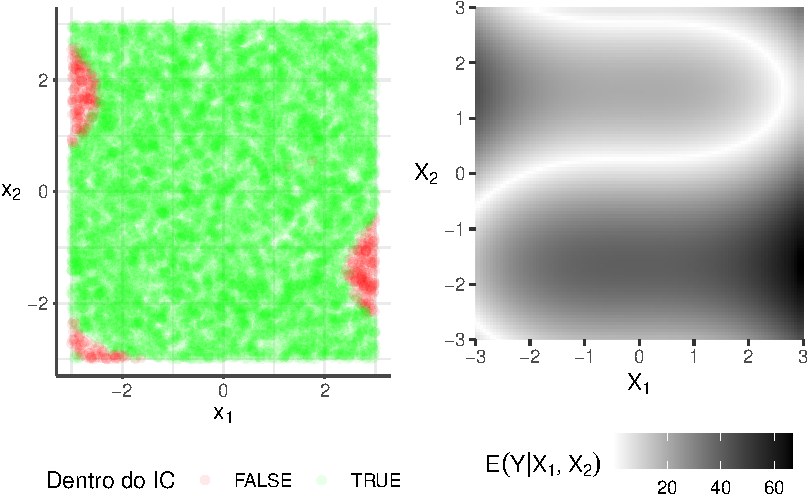
\includegraphics{lista1-resolucao_files/figure-pdf/fig-intervaloconfianca-1.pdf}

}

\caption{\label{fig-intervaloconfianca}Pontos contidos nos intervalos de
confiança de 95\% para o Modelo Linear 1.}

\end{figure}%

~

Para comparação, é feito o mesmo gráfico para os intervalos de confiança
da rede neural. Em comparação ao caso anterior, há um padrão que se
assemelha ao gráfico da esperança condicional. Parte do vale no senóide
não é capturado, especificamente os próximos e pertencentes ao terceiro
quadrante, assim como valores de alta esperança no quarto quadrante.

\begin{Shaded}
\begin{Highlighting}[]
\NormalTok{tabela\_withinrn }\SpecialCharTok{\%\textgreater{}\%}
  \FunctionTok{mutate}\NormalTok{(}\AttributeTok{x1 =}\NormalTok{ dados\_test}\SpecialCharTok{$}\NormalTok{x1.obs,}
         \AttributeTok{x2 =}\NormalTok{ dados\_test}\SpecialCharTok{$}\NormalTok{x2.obs) }\SpecialCharTok{\%\textgreater{}\%}
  \FunctionTok{ggplot}\NormalTok{(}\FunctionTok{aes}\NormalTok{(x1, x2, }\AttributeTok{color =}\NormalTok{ within))}\SpecialCharTok{+}
  \FunctionTok{scale\_color\_manual}\NormalTok{(}\AttributeTok{values =} \FunctionTok{c}\NormalTok{(}\StringTok{"green"}\NormalTok{, }\StringTok{"red"}\NormalTok{)) }\SpecialCharTok{+}
  \FunctionTok{geom\_point}\NormalTok{(}\AttributeTok{alpha =} \FloatTok{0.12}\NormalTok{)}\SpecialCharTok{+}
  \FunctionTok{theme\_bw}\NormalTok{()}\SpecialCharTok{+}
  \FunctionTok{labs}\NormalTok{(}\AttributeTok{x =} \FunctionTok{TeX}\NormalTok{(}\StringTok{"$x\_1$"}\NormalTok{), }\AttributeTok{y =} \FunctionTok{TeX}\NormalTok{(}\StringTok{"$x\_2$"}\NormalTok{), }\AttributeTok{color =} \StringTok{"Dentro do IC"}\NormalTok{)}\SpecialCharTok{+}
  \FunctionTok{theme}\NormalTok{(}\AttributeTok{panel.border =} \FunctionTok{element\_blank}\NormalTok{(), }\CommentTok{\# Remove all panel borders}
    \AttributeTok{axis.line =} \FunctionTok{element\_line}\NormalTok{(}\AttributeTok{color =} \StringTok{"\#474747"}\NormalTok{), }\CommentTok{\# Add axis lines}
    \AttributeTok{axis.ticks.x =} \FunctionTok{element\_line}\NormalTok{(}\AttributeTok{color =} \StringTok{"\#474747"}\NormalTok{), }\CommentTok{\# X axis ticks}
    \AttributeTok{axis.ticks.y =} \FunctionTok{element\_line}\NormalTok{(}\AttributeTok{color =} \StringTok{"\#474747"}\NormalTok{), }\CommentTok{\# Y axis ticks}
    \AttributeTok{axis.ticks.length =} \FunctionTok{unit}\NormalTok{(}\FloatTok{0.05}\NormalTok{, }\StringTok{"cm"}\NormalTok{), }\CommentTok{\# Control tick length}
    \AttributeTok{legend.position =} \StringTok{"bottom"}\NormalTok{,}
    \AttributeTok{axis.title.y =} \FunctionTok{element\_text}\NormalTok{(}\AttributeTok{angle =} \DecValTok{0}\NormalTok{, }\AttributeTok{vjust =} \FloatTok{0.5}\NormalTok{),}
    \AttributeTok{aspect.ratio =} \DecValTok{1}\NormalTok{)}
\end{Highlighting}
\end{Shaded}

\begin{figure}[H]

\centering{

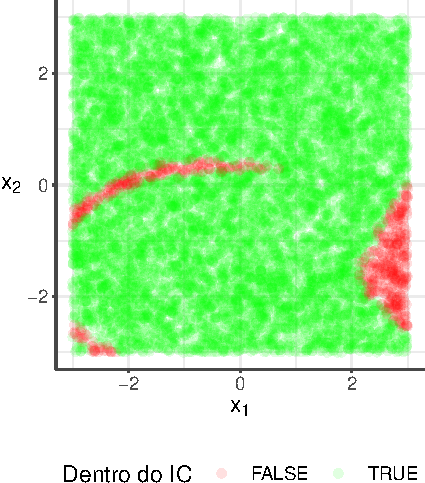
\includegraphics{lista1-resolucao_files/figure-pdf/fig-intervaloconfiancarede-1.pdf}

}

\caption{\label{fig-intervaloconfiancarede}Pontos contidos nos
intervalos de confiança de 95\% para a Rede Neural.}

\end{figure}%

\section{Lições aprendidas}\label{liuxe7uxf5es-aprendidas}

É muito positivo construir funções que retornam listas com os resultados
de cada etapa do algoritmo. Isso facilita a depuração e a compreensão do
código. Além disso, é importante testar cada função separadamente para
garantir que ela está retornando o resultado esperado.

Frequentemente quando avançava um item, percebia que poderia incrementar
funções anteriores que já retornavam internamente vetores que seriam
usados futuramente. Dessa forma, é possível utilizar listas para fazer
referencias fáceis a componentes de cada etapa e evitar repetições
desnecessárias de cálculos, reduzindo o custo computacional da lista
como um todo.

A utilização de \texttt{cache:\ true} na seção YAML do documento é muito
útil para economizar tempo para renderizar versões incrementadas do
documento, especialmente no caso de termos que executar várias vezes
cálculos custosos como o back propagation --- Isso foi escrito quando eu
usava o processo de \emph{back-propagation} dentro de um \texttt{for}.

O tempo de processamento foi reduzido de 10 minutos a 5s usando contas
matriciais. No entanto, tive muitos problemas na hora de converter o
código. Uma revisão bem detalhada teve que ser feita para identificar
pequenos problemas de matrizes transpostas.

Para os gráficos, poderia ter sido mais econômico em termos de linhas de
código se tivesse montado uma função para toda a configuração do
\texttt{theme()}.



\end{document}
